%------------------------------------------------------------------------------------
\section{Karate Do}
\label{sec:Karate-Do}
El Karate Do, en todas sus diferentes formas, encuentra sus orígenes en un sólo lugar, las islas Ryukyu fuera de la costa de Japón. Lo que se sabe de uno de los sistemas de entrenamiento de auto defensa y disciplina más practicados en el mundo es el resultado de siglos de desarrollo. \\

El Karate Do es un arte marcial tradicional en el que se coordina la fuerza, la respiración, el equilibrio y la postura, el correcto giro de cadera y la conexión conjunta de músculos y extremidades, trasladando gran parte del peso corporal y del centro de gravedad al impacto. Se caracteriza por el empleo de golpes de puño y patadas, aunque no restringe su repertorio sólo a ellos. Normalmente, un entrenamiento de Karate Do se divide en 5 partes que son: el calentamiento, los ejercicios de resistencia, la técnica, las Katas y el Kumite (o combate); el presente trabajo está enfocado en el aprendizaje de la técnica del Karate Do, por lo que se verán contemplados los ejercicios de calentamiento y los movimientos de técnica. \\

En la actualidad existen diferentes estilos en la enseñanza del Karate Do, todos basados en la técnica original, pero normalmente cambiando los métodos de enseñanza dependiendo de las regiones o incluso de cada instructor. Para el caso del presente trabajo terminal, se tiene el apoyo y asesoría del experto Moisés Gachúz Mendoza cuyo grado es de Cinta Negra 5to Dan registrado en la Federación Mexicana de Karate Do desde el 2005.
%------------------------------------------------------------------------------------
\subsection{Calentamiento}
\label{sec:Calentamiento}
El calentamiento es un aspecto importante para cualquier rutina de ejercicios. Realizar ejercicios de calentamiento antes de estiramientos, calienta la temperatura del cuerpo, lo cual incrementa el flujo de sangre en los músculos y los hace más flexibles. El calentamiento también protege al corazón, ya que las personas que calientan por al menos dos minutos antes de una rutina de ejercicios reducen su riesgo de alta presión sanguínea e incrementa el flujo de oxígeno en el corazón. El calentamiento debe ser la primera actividad realizada antes de hacer estiramientos, ejercicio cardiovascular o entrenamiento de resistencia \cite{Nall}.\\

Existen ejercicios de calentamiento recomendados especialmente para cada tipo de actividad física o deportiva, el Karate Do es un deporte que no se enfoca en una sola actividad, sino que tiene una combinación de varias, como los ejercicios de resistencia, el estiramiento o los ejercicios cardiovasculares; es por ello que para el presente trabajo terminal se proponen rutinas de entrenamiento con los siguientes ejercicios de calentamiento, Figura \ref{fig:Musculos_Cuello} - Figura \ref{fig:Musculos_Estiramiento3}, indicados como parte del Programa Nacional de Activación Física de la CONADE \cite{CONADE}:

\clearpage

\begin{figure}[H]
	\centering
	\subfloat[Flexión lateral del cuello, izquierdo y derecho]{
		\label{fig:Cuello_Frontal}
		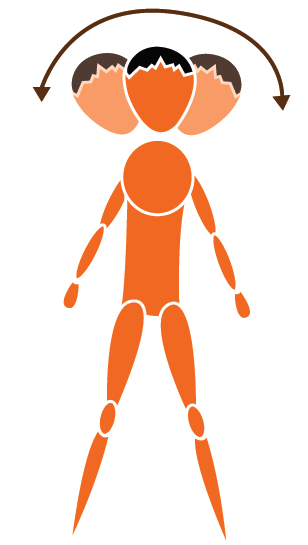
\includegraphics[width=4.5cm, height=8cm]{./Figuras/Calentamiento/1_Flexion_lateral_del_cuello}}
	\subfloat[Flexión del cuello al frente y extensión del cuello atrás]{
		\label{fig:Cuello_Lateral}
		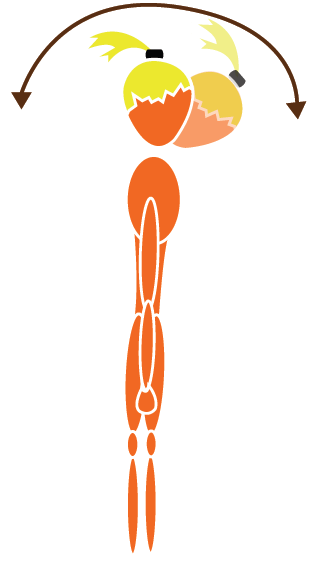
\includegraphics[width=5.5cm, height=8cm]{./Figuras/Calentamiento/2_Flexion_del_cuello_al_frente}}
	\caption{Músculos de cuello}
	\label{fig:Musculos_Cuello}
\end{figure}

\begin{figure}[H]
	\begin{center}
		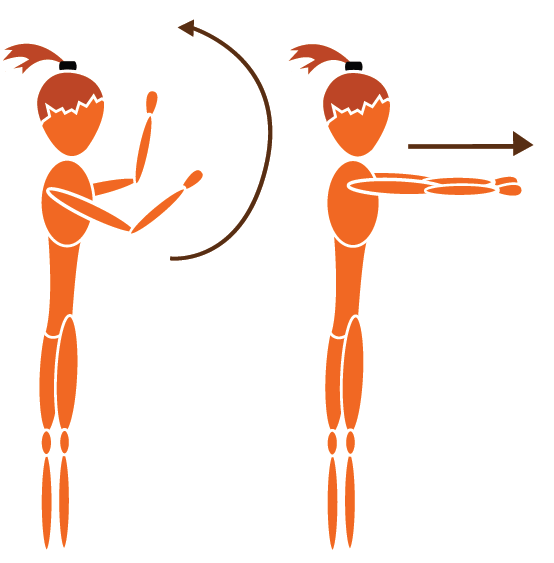
\includegraphics[width=8cm, height=8cm]{./Figuras/Calentamiento/7_Flexion_del_codo}\\
		Flexión y extensión del codo
	\end{center}
	\caption{Músculos del brazo}
	\label{fig:Musculos_Brazo}
\end{figure}

\begin{figure}[H]
	\centering
	\subfloat[Flexión y extensión del tronco(enfrente y atrás)]{
		\label{fig:Tronco_Frontal}
		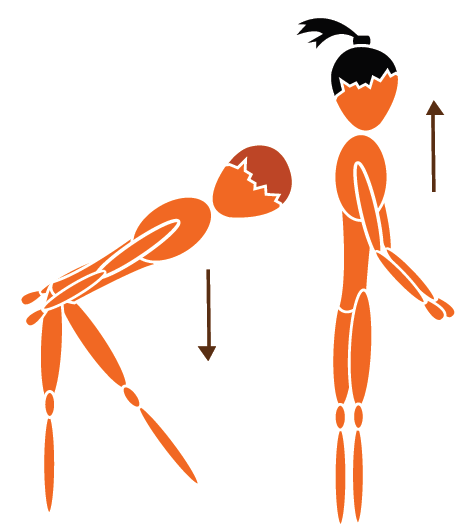
\includegraphics[width=7cm, height=8cm]{./Figuras/Calentamiento/12_Flexion_del_tronco}}
	\subfloat[Flexión del tronco izquierdo y derecho]{
		\label{fig:Tronco_Lateral}
		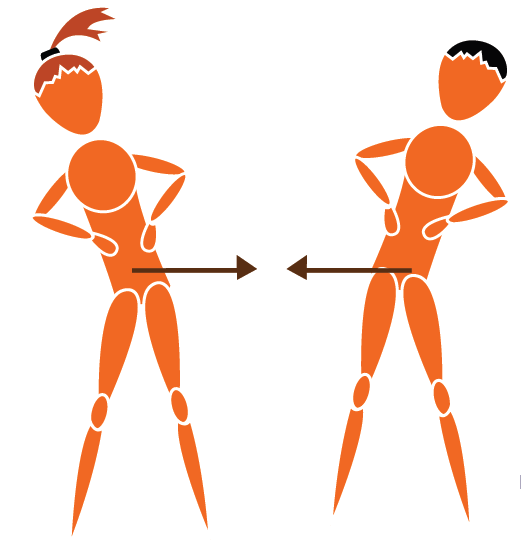
\includegraphics[width=5.5cm, height=8cm]{./Figuras/Calentamiento/13_Flexion_lateral_del_tronco}}
	\caption{Músculos de la cadera}
	\label{fig:Musculos_Cadera}
\end{figure}

\begin{figure}[H]
	\centering
	\subfloat[Flexión y extensión de rodilla]{
		\label{fig:Piernas_Frontal}
		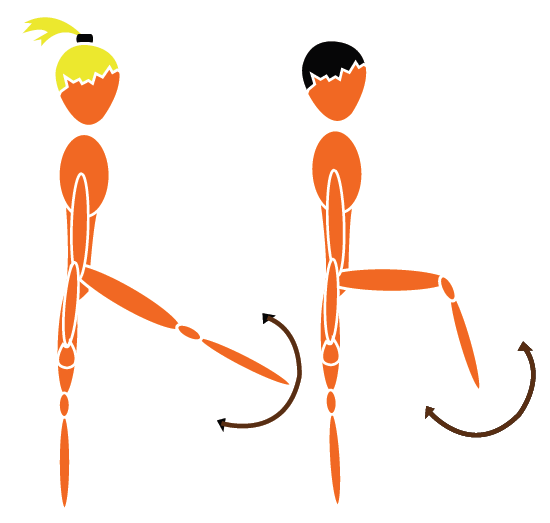
\includegraphics[width=8cm, height=8cm]{./Figuras/Calentamiento/15_Flexion_de_la_rodilla}}
	\subfloat[Abrir y cerrar las piernas derecha e izquierda]{
		\label{fig:Piernas_Lateral}
		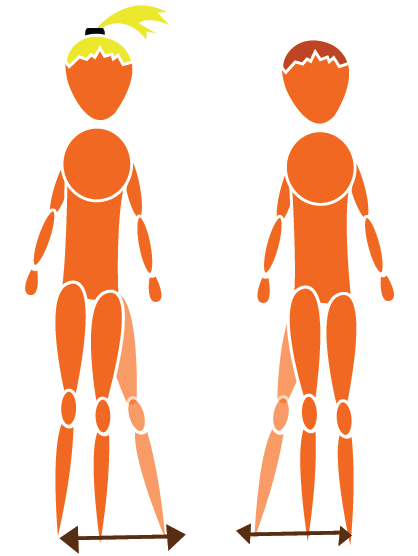
\includegraphics[width=5.5cm, height=8cm]{./Figuras/Calentamiento/16_Abrir_piernas}}
	\caption{Músculos de la pierna}
	\label{fig:Musculos_Pierna}
\end{figure}

\begin{figure}[H]
	\centering
	\subfloat[Estiramiento de músculos posteriores de la pierna]{
		\label{fig:Musculos_Estiramiento1}
		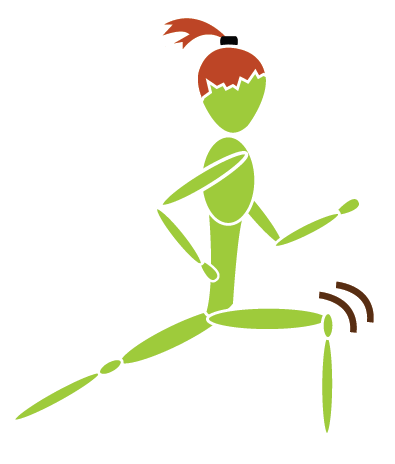
\includegraphics[width=5.5cm, height=8cm]{./Figuras/Calentamiento/28_Estiramiento_de_musculos_de_la_pierna}}
	\subfloat[Estiramiento del músculo de la pierna]{
		\label{fig:Musculos_Estiramiento2}
		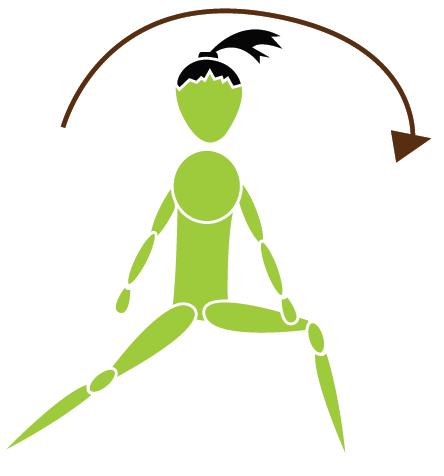
\includegraphics[width=5.5cm, height=8cm]{./Figuras/Calentamiento/29_Estiramiento_del_musculo_de_la_pierna}}
	\caption{Estiramientos de pierna}
	\label{fig:Estiramientos_Pierna}
\end{figure}

\begin{figure}[H]
	\begin{center}
		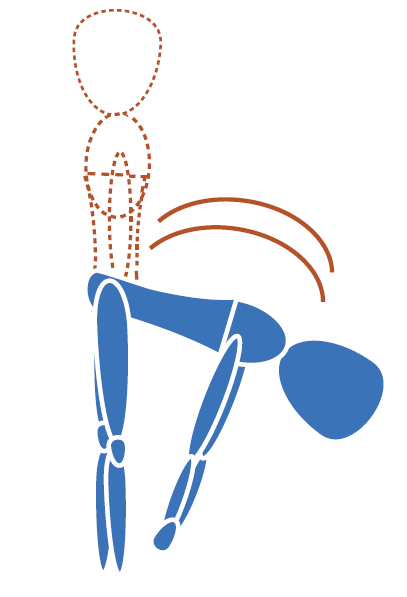
\includegraphics[width=5.5cm, height=8cm]{./Figuras/Calentamiento/44_lab_Flexion_de_tronco_al_frente}\\
		Separación de las piernas a la altura de los hombros, se flexiona el tronco tocando la punta de los pies
	\end{center}
	\caption{Estiramiento}
	\label{fig:Musculos_Estiramiento3}
\end{figure}

%-----------------------------------------------------------------------------
\subsubsection{Descripción de ejercicios}
La siguiente tabla muestra la lista de los ejercicios de calentamiento propuestos en la herramienta, describiendo la manera de realizarse y su utilidad en la realización de la técnica del Karate Do.

\begin{table}[H]
\centering
\begin{tabular}{| p{3 cm} | p{4 cm} | p{4 cm} | p{4 cm} |}
\hline
\rowcolor[rgb]{0.529412, 0.807843, 0.980392} {\textbf{Parte del cuerpo}} & {\textbf{Postura}} & {\textbf{Descripción}} & {\textbf{Técnica de Karate Do}}\\
\hline
\textbf{Calentamiento de músculos del cuello} &  Brazos extendidos a los costados.
Piernas ligeramente abiertas a la altura de los hombros. & Flexión lateral del cuello, hacia la izquierda y hacia la derecha. & Es necesario para realizar posiciones de manera precisa.\\
\hline
\textbf{Calentamiento de músculos del cuello} & Brazos extendidos a los costados.
Piernas ligeramente abiertas a la altura de los hombros. & Flexión del cuello hacia el frente y extensión del cuello hacia atrás. & Es necesario para realizar posiciones de manera precisa.\\
\hline
\textbf{Calentamiento de músculos del brazo} & Piernas ligeramente abiertas a la altura de los hombros.
Brazos levantados a la altura de los hombros. & Flexión y extensión de los codos. & Es necesario para realizar posiciones, ataques con brazo y defensas de manera precisa.\\
\hline
\textbf{Calentamiento de músculos de cadera} & Piernas separadas, superando la posición de los hombros. & Flexión y extensión del tronco, hacia enfrente y atrás. & Es necesario para realizar posiciones y ataques con pierna de manera precisa.\\		
\hline
\textbf{Calentamiento de músculos de cadera} & Piernas separadas, superando la posición de los hombros. & Flexión del tronco hacia los lados derecho e izquierdo. & Es necesario para realizar posiciones y ataques con pierna de manera precisa.\\
\hline
\textbf{Calentamiento de músculos de la pierna} & Una pierna en el suelo y la otra pierna levantada a la altura de la cadera. & Flexión y extensión de la rodilla de la pierna levantada. & Es necesario para realizar posiciones y ataques con pierna de manera precisa.\\
\hline
\textbf{Calentamiento de músculos de la pierna} & Piernas ligeramente abiertas a la altura de los hombros. & Abrir y cerrar las piernas (una a la vez) haciendo movimientos de derecha a izquierda.& Es necesario para realizar posiciones y ataques con pierna de manera precisa.\\
\hline


\end{tabular}
%\caption{Descripción de ejercicios de calentamiento}
\label{tab:DEC}
\end{table} 

\begin{table}[H]
\centering
\begin{tabular}{| p{3 cm} | p{4 cm} | p{4 cm} | p{4 cm} |}
\hline
\textbf{Estiramiento de músculos de la pierna} & Una pierna flexionada hacia el frente y la otra estirada hacia atrás. & Mantener la posición por unos segundos. & Es necesario para realizar posiciones de manera precisa, así como ataques con pierna con mayor fuerza y alcance.\\
\hline	
\textbf{Estiramiento de músculos de la pierna} & Con el cuerpo de frente se estira una pierna y la otra se flexiona. & Mantener la posición por unos segundos, recargando la mayor parte del peso sobre la pierna flexionada. & Es necesario para realizar posiciones de manera precisa, así como ataques con pierna con mayor fuerza y alcance.\\
\hline
\textbf{Estiramiento de piernas y cadera} & Piernas ligeramente separadas a la altura de los hombros. & Flexionar el tronco hacia enfrente, tocando la punta de los pies con las manos.
Mantener la posición por unos segundos. & Es necesario para realizar posiciones de manera precisa, así como ataques con pierna con mayor fuerza y alcance.\\
\hline
\end{tabular}
\caption{Descripción de ejercicios de calentamiento}
\label{tab:DEC2}
\end{table} 

%------------------------------------------------------------------------------------
\subsection{Técnica}
La técnica es un procedimiento o conjunto de reglas, normas o protocolos que tienen como objetivo obtener un resultado determinado.
Para el caso del Karate Do, la técnica hace referencia al conjunto de movimientos propios de dicho deporte, como son los ataques, las defensas, las posiciones , Katas y Kumite (combate); el presente trabajo terminal está enfocado en la técnica inicial de cinta blanca la cual contempla los primeros tres, tomando como referencia los movimientos específicos que se muestran a continuación, de la Figura \ref{fig:Posiciones1} a la Figura \ref{fig:Ataques2}:

\begin{figure}[H]
	\centering
	\subfloat[Musubi - dachi frontal]{
		\label{fig:Musubidachi_Frontal}
		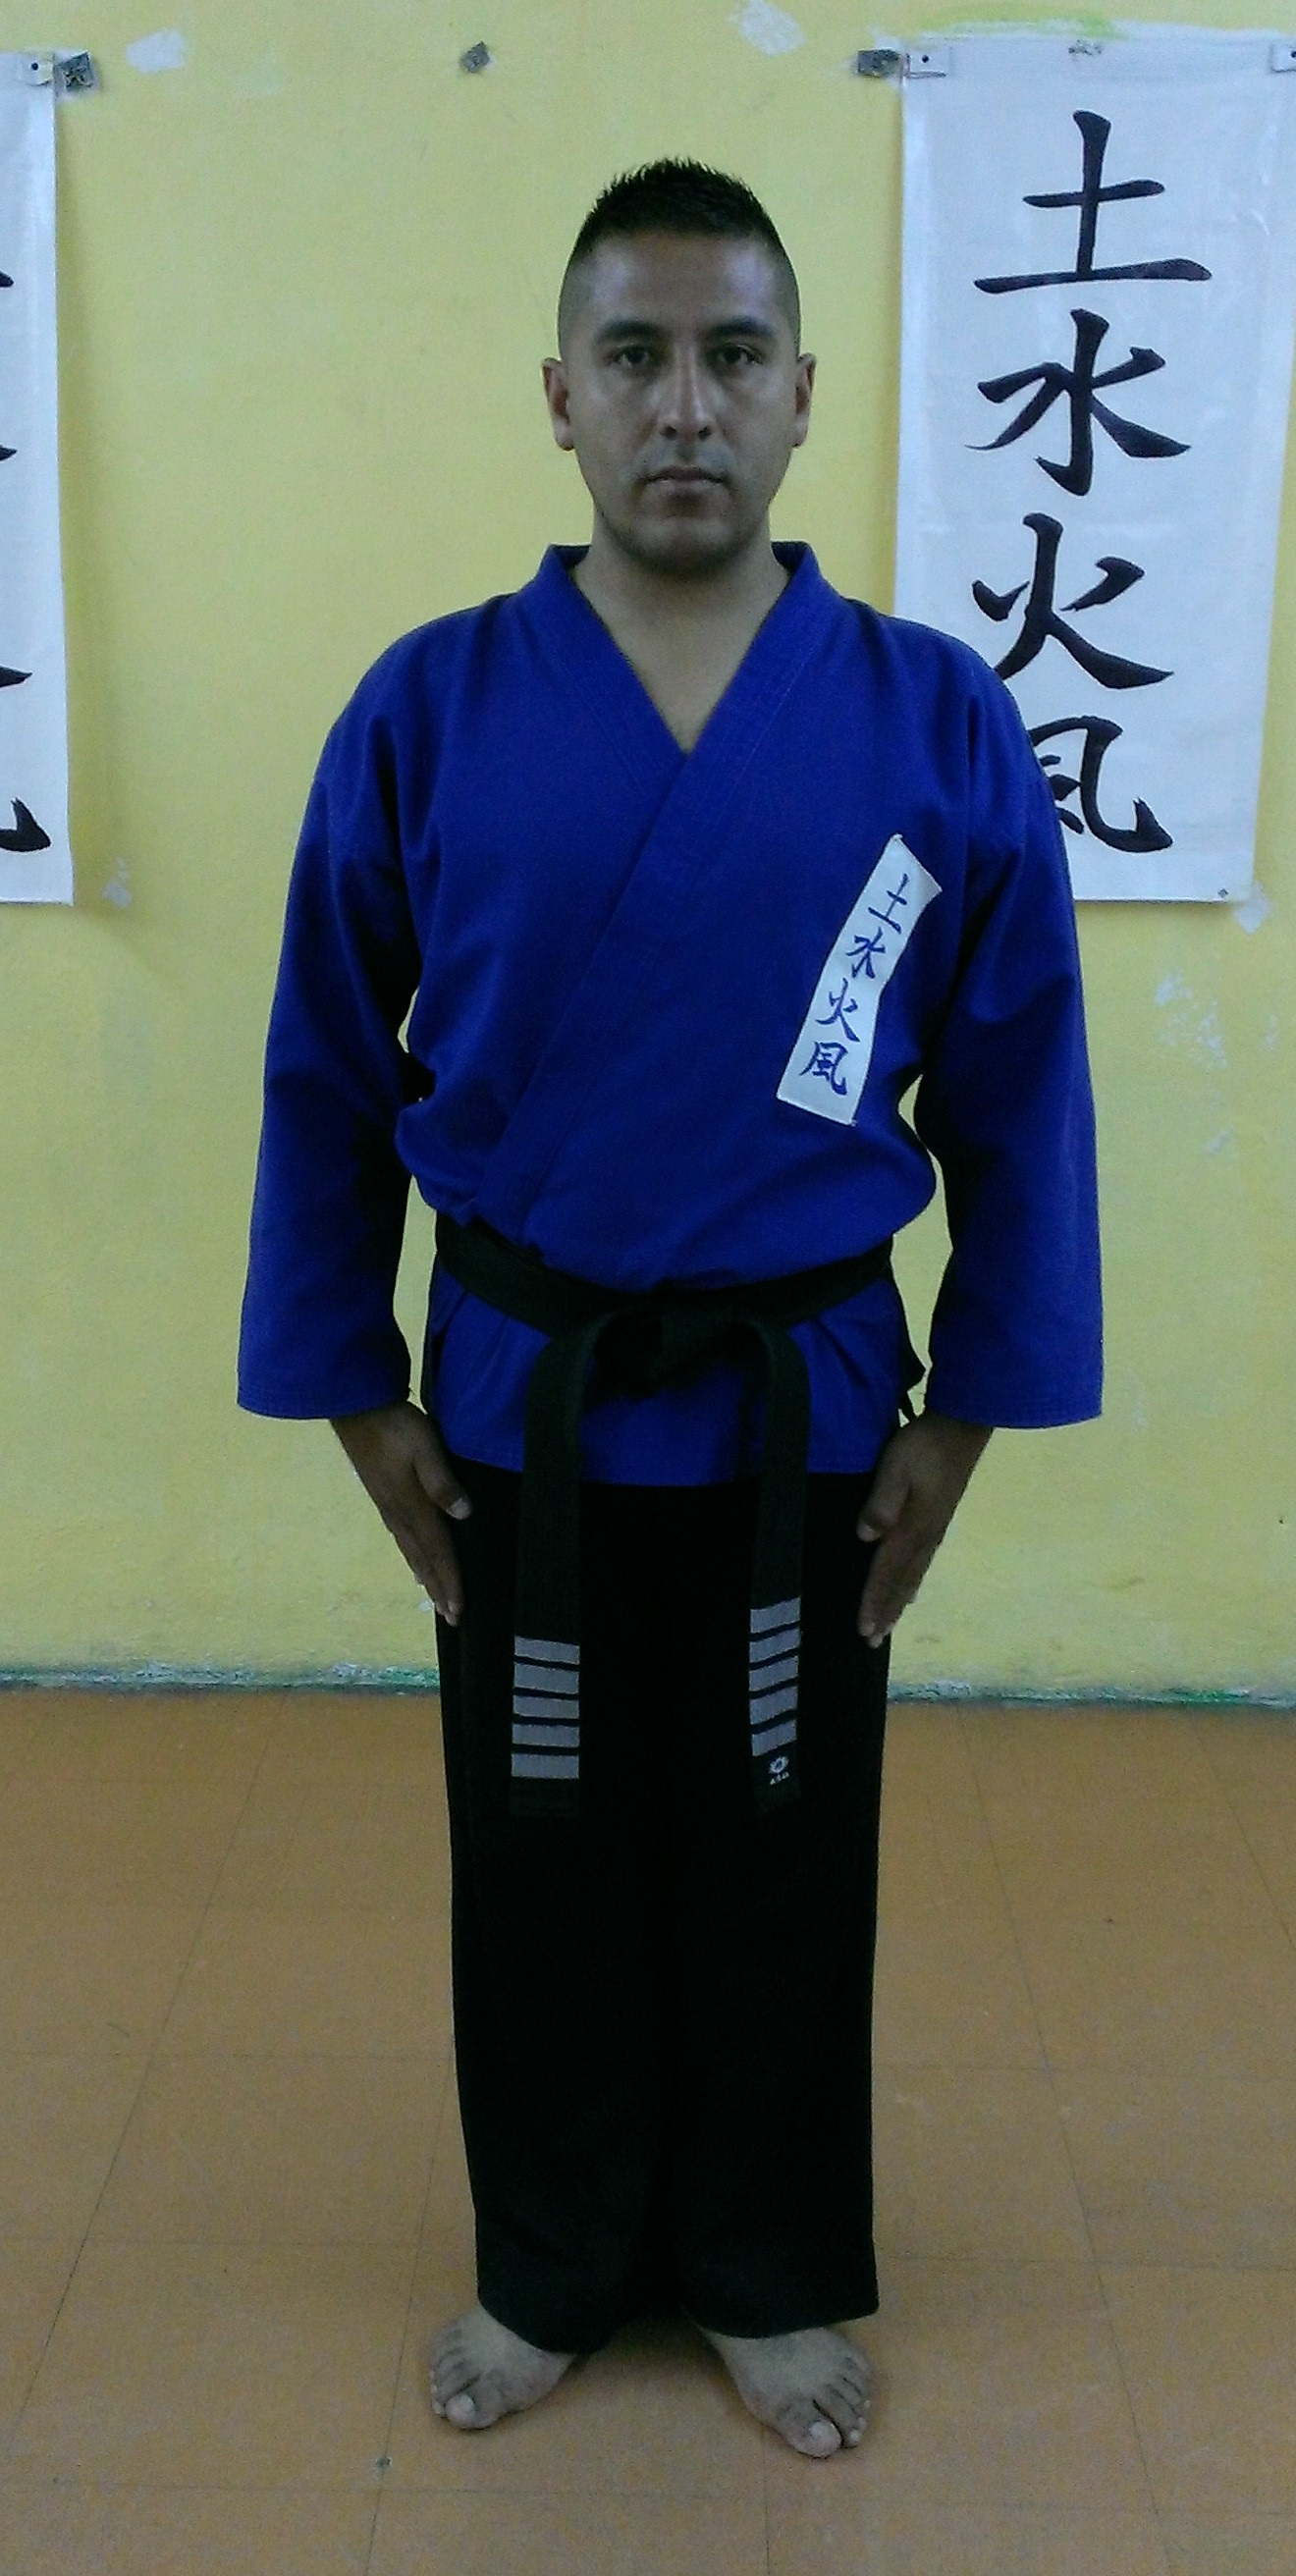
\includegraphics[width=4.5cm, height=8cm]{./Figuras/Tecnica/Musubidachi_Frontal}}
	\subfloat[Hachiji - dachi frontal]{
		\label{fig:Hachijidachi_Frontal}
		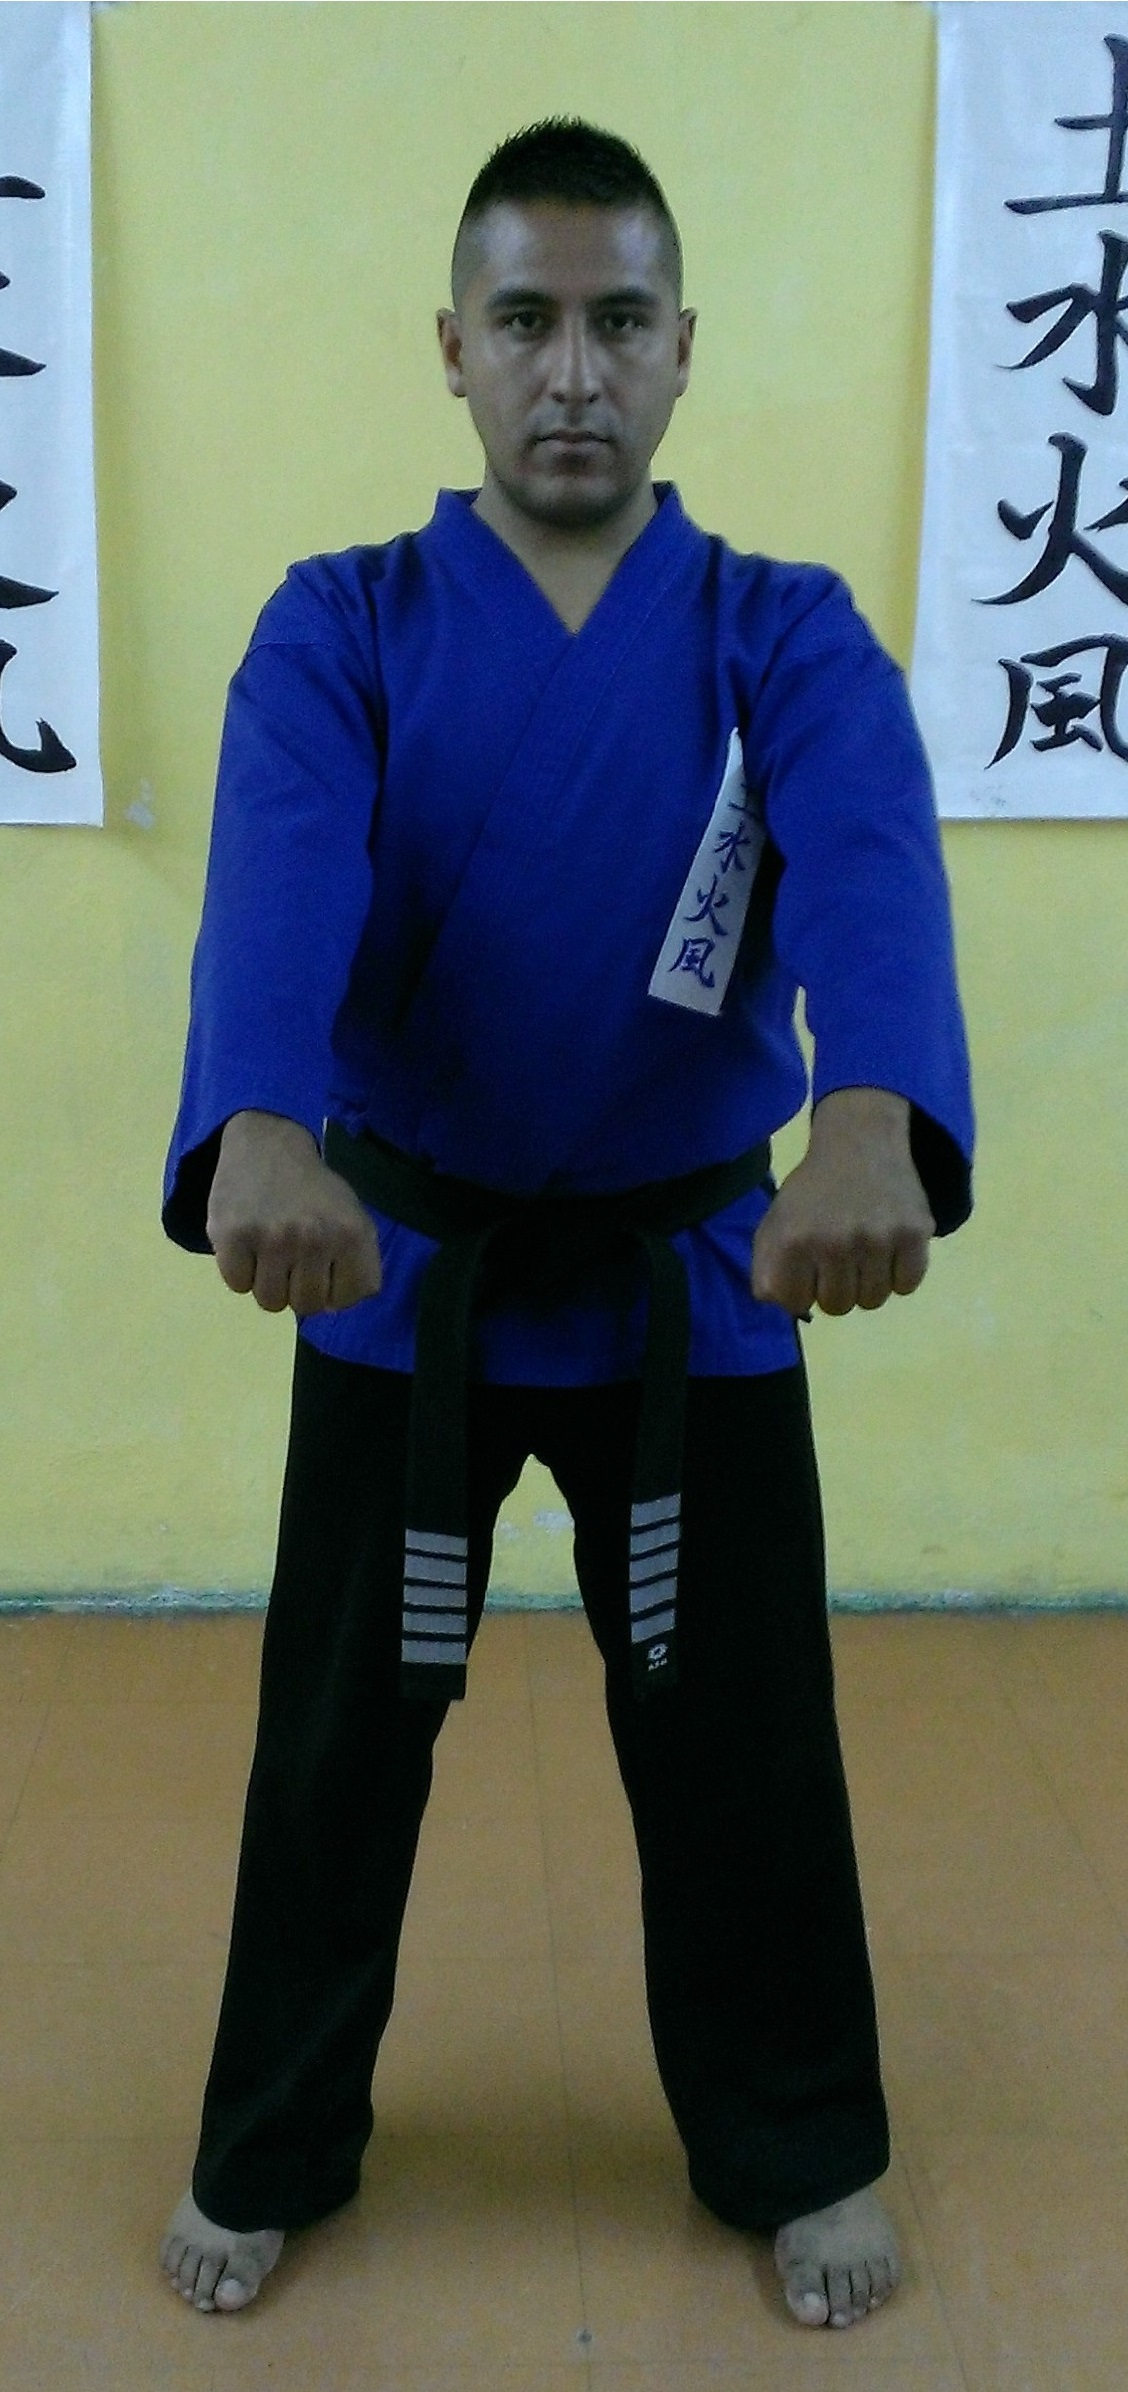
\includegraphics[width=4.5cm, height=8cm]{./Figuras/Tecnica/Hachijidachi_Frontal}}
	\caption{Posiciones Musubi - dachi y Hachiji - dachi }
	\label{fig:Posiciones1}
\end{figure}

\begin{figure}[H]
	\centering
	\subfloat[Posición Senkuntsu - dachi frontal]{
		\label{fig:Senkuntsudachi_Frontal}
		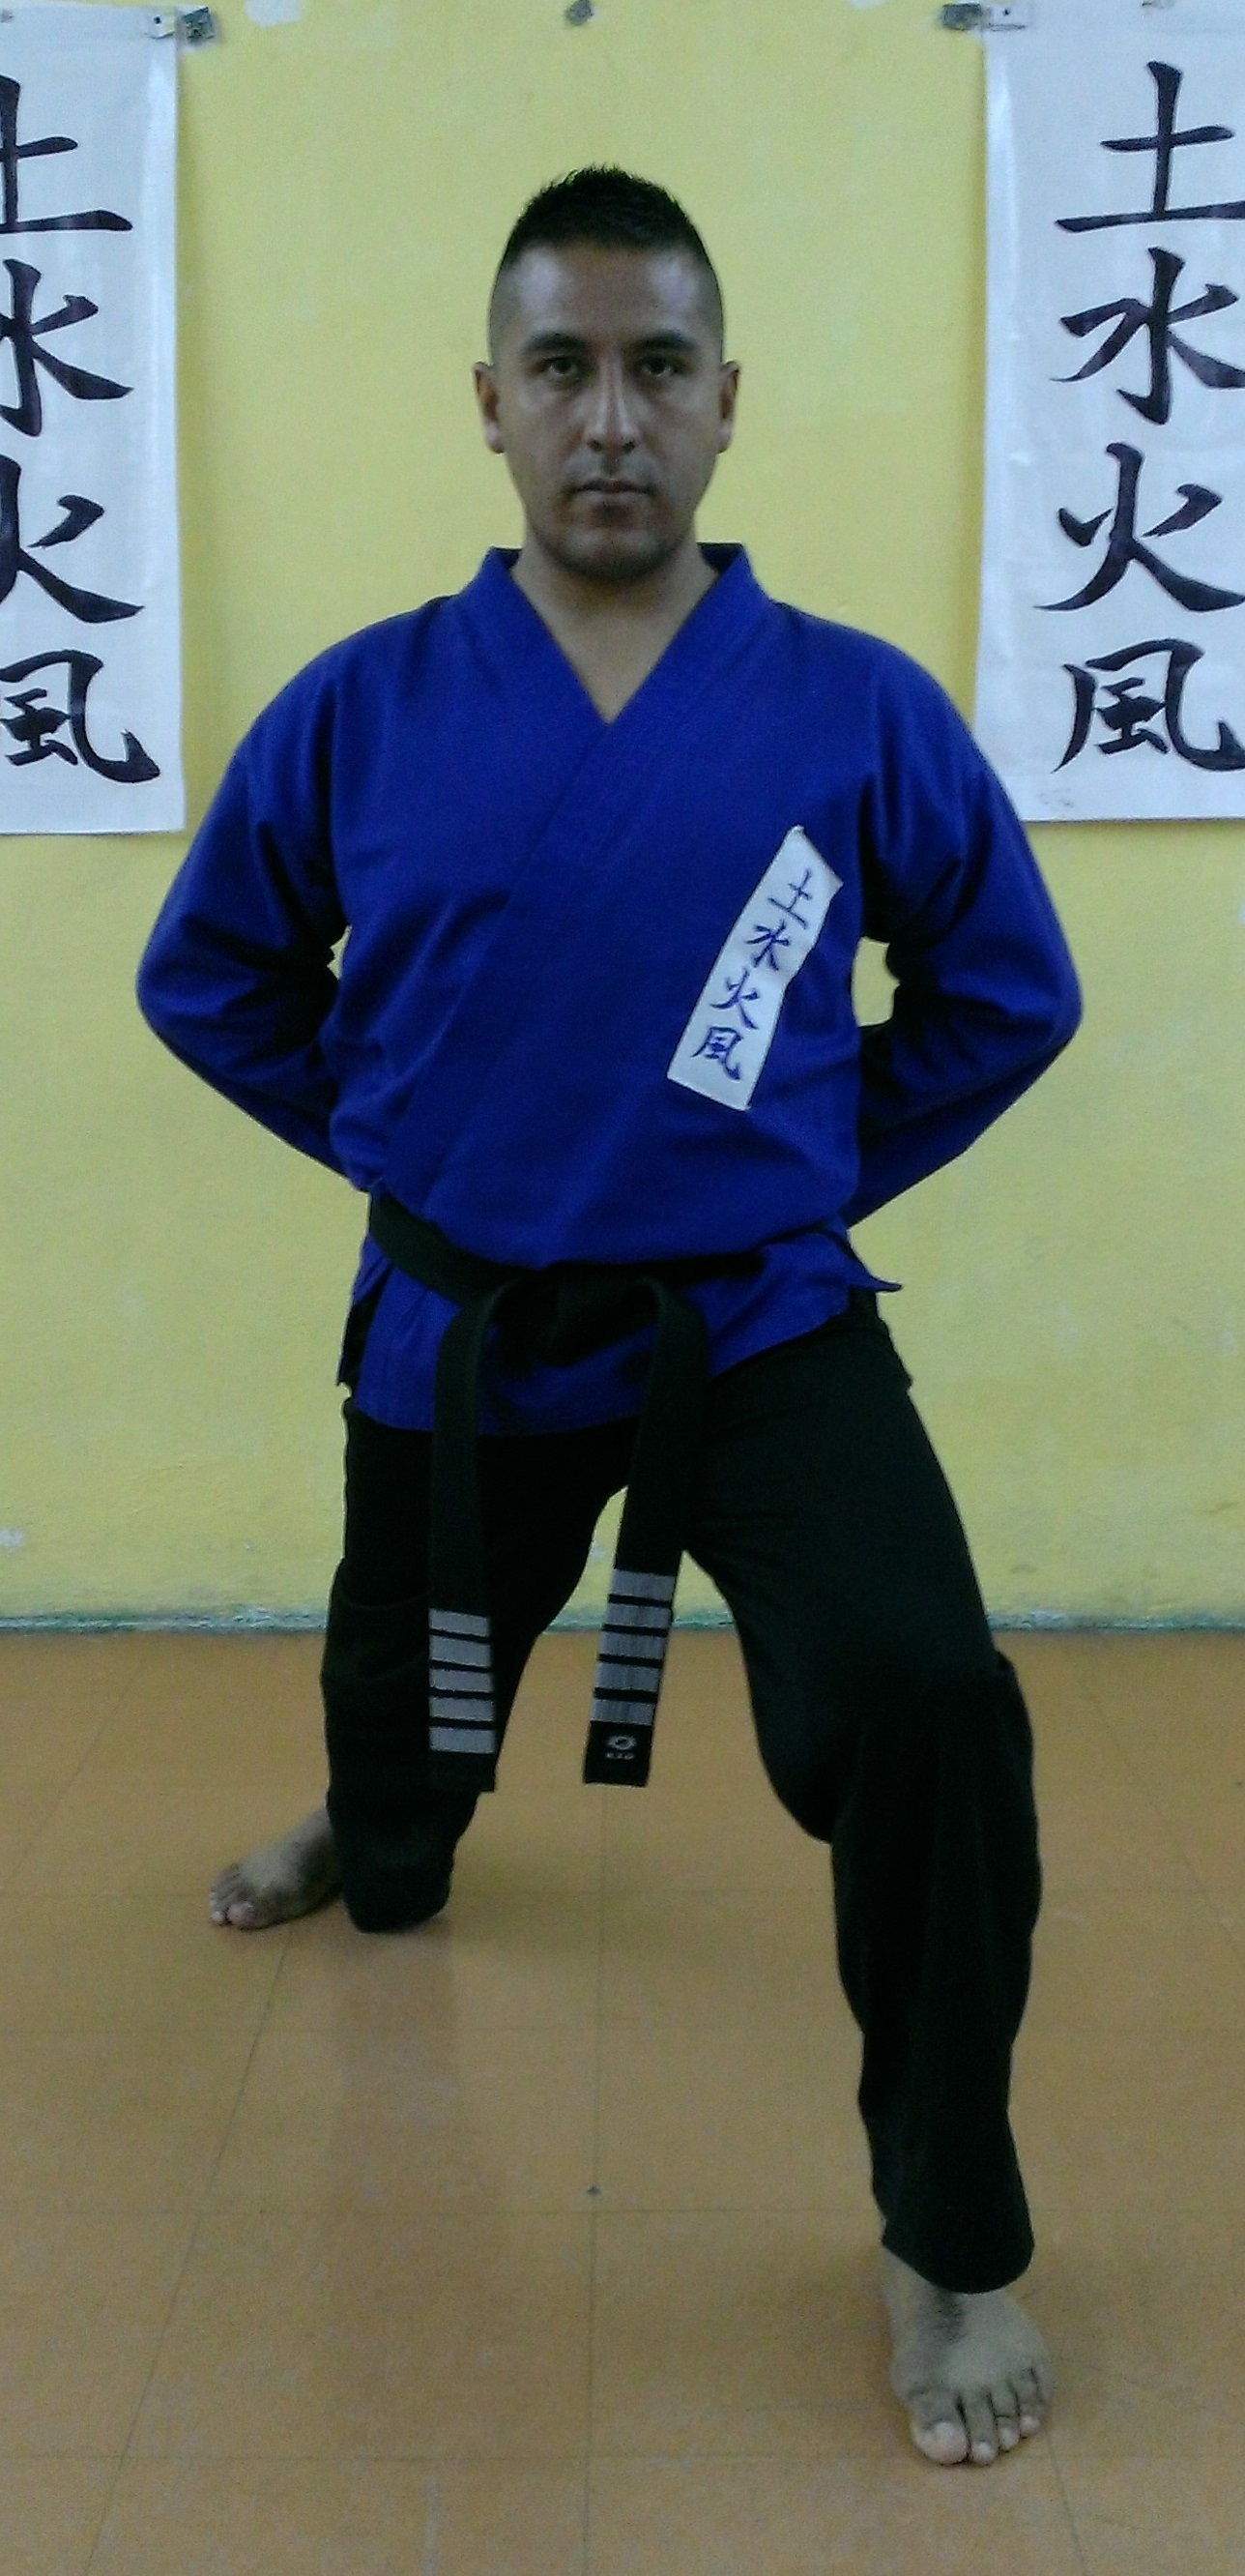
\includegraphics[width=4.5cm, height=8cm]{./Figuras/Tecnica/Senkuntsudachi_Frontal}}
	\subfloat[Posición Senkuntsu - dachi lateral]{
		\label{fig:Senkuntsudachi_Lateral}
		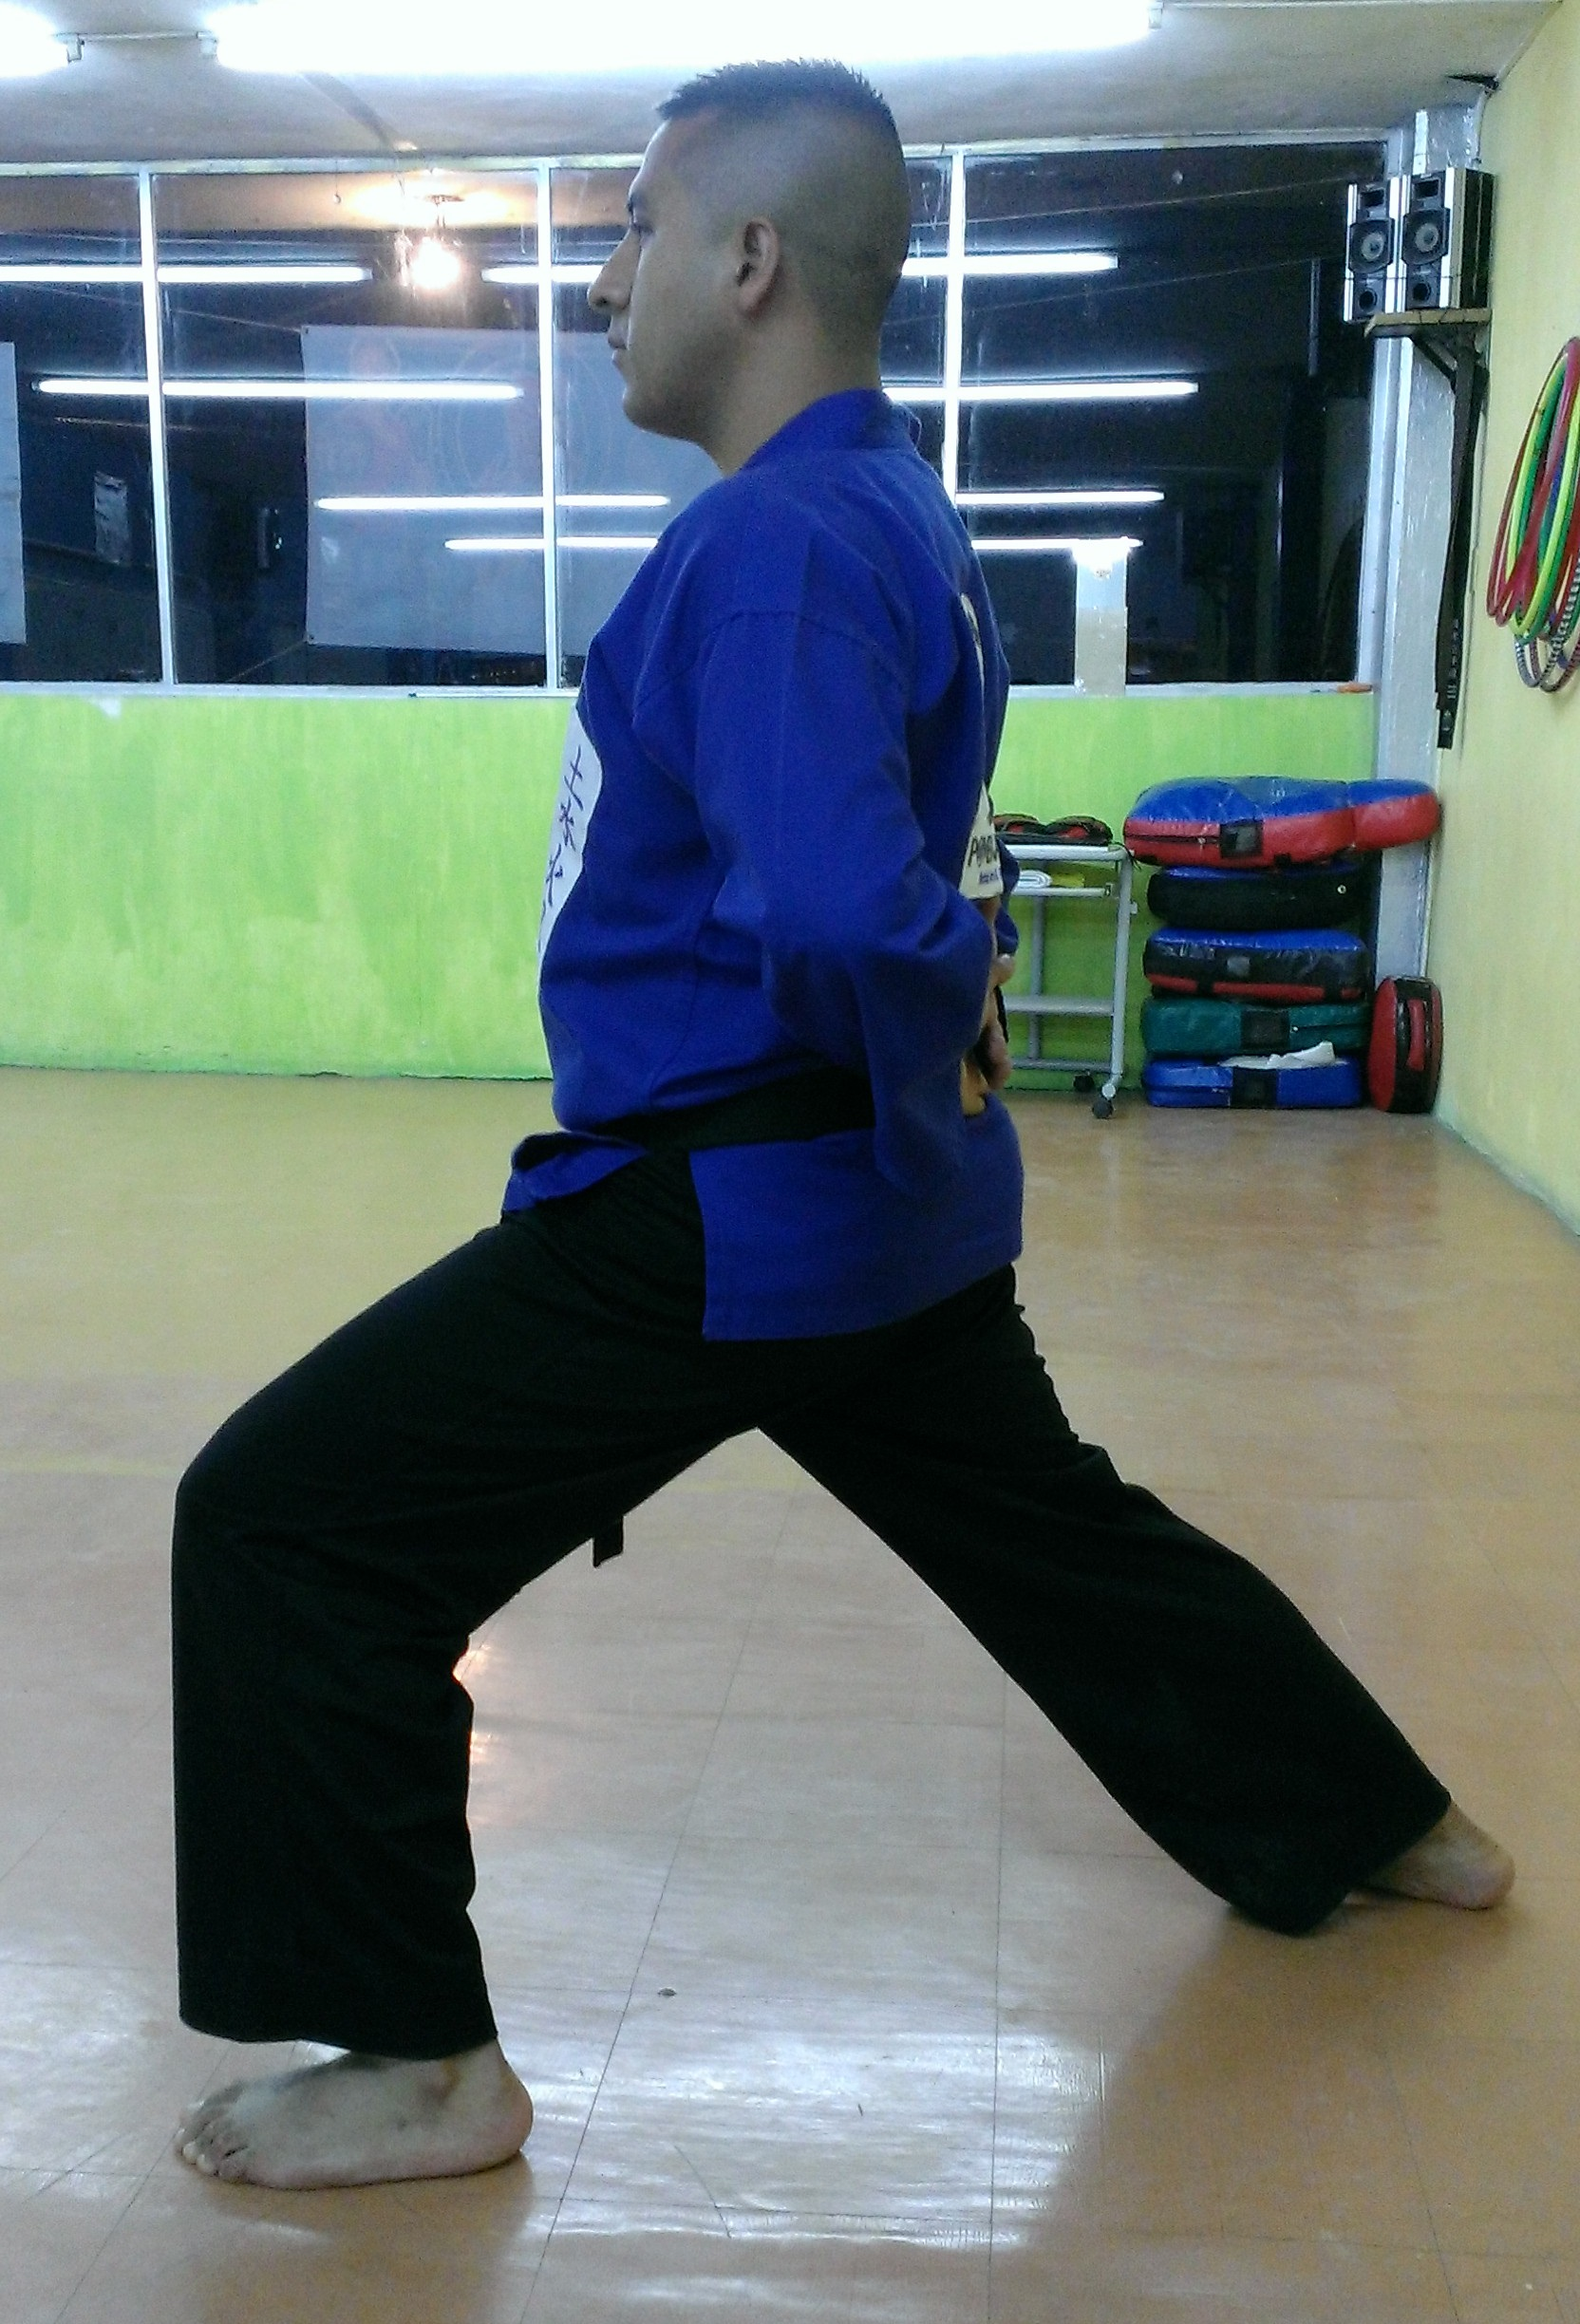
\includegraphics[width=5.5cm, height=8cm]{./Figuras/Tecnica/Senkuntsudachi_Lateral}}
	\caption{Posición Senkuntsu - dachi}
	\label{fig:Posiciones2}
\end{figure}

\begin{figure}[H]
	\centering
	\subfloat[Defensa Gedan Barai Uke frontal]{
		\label{fig:GedanBaraiUke_Frontal}
		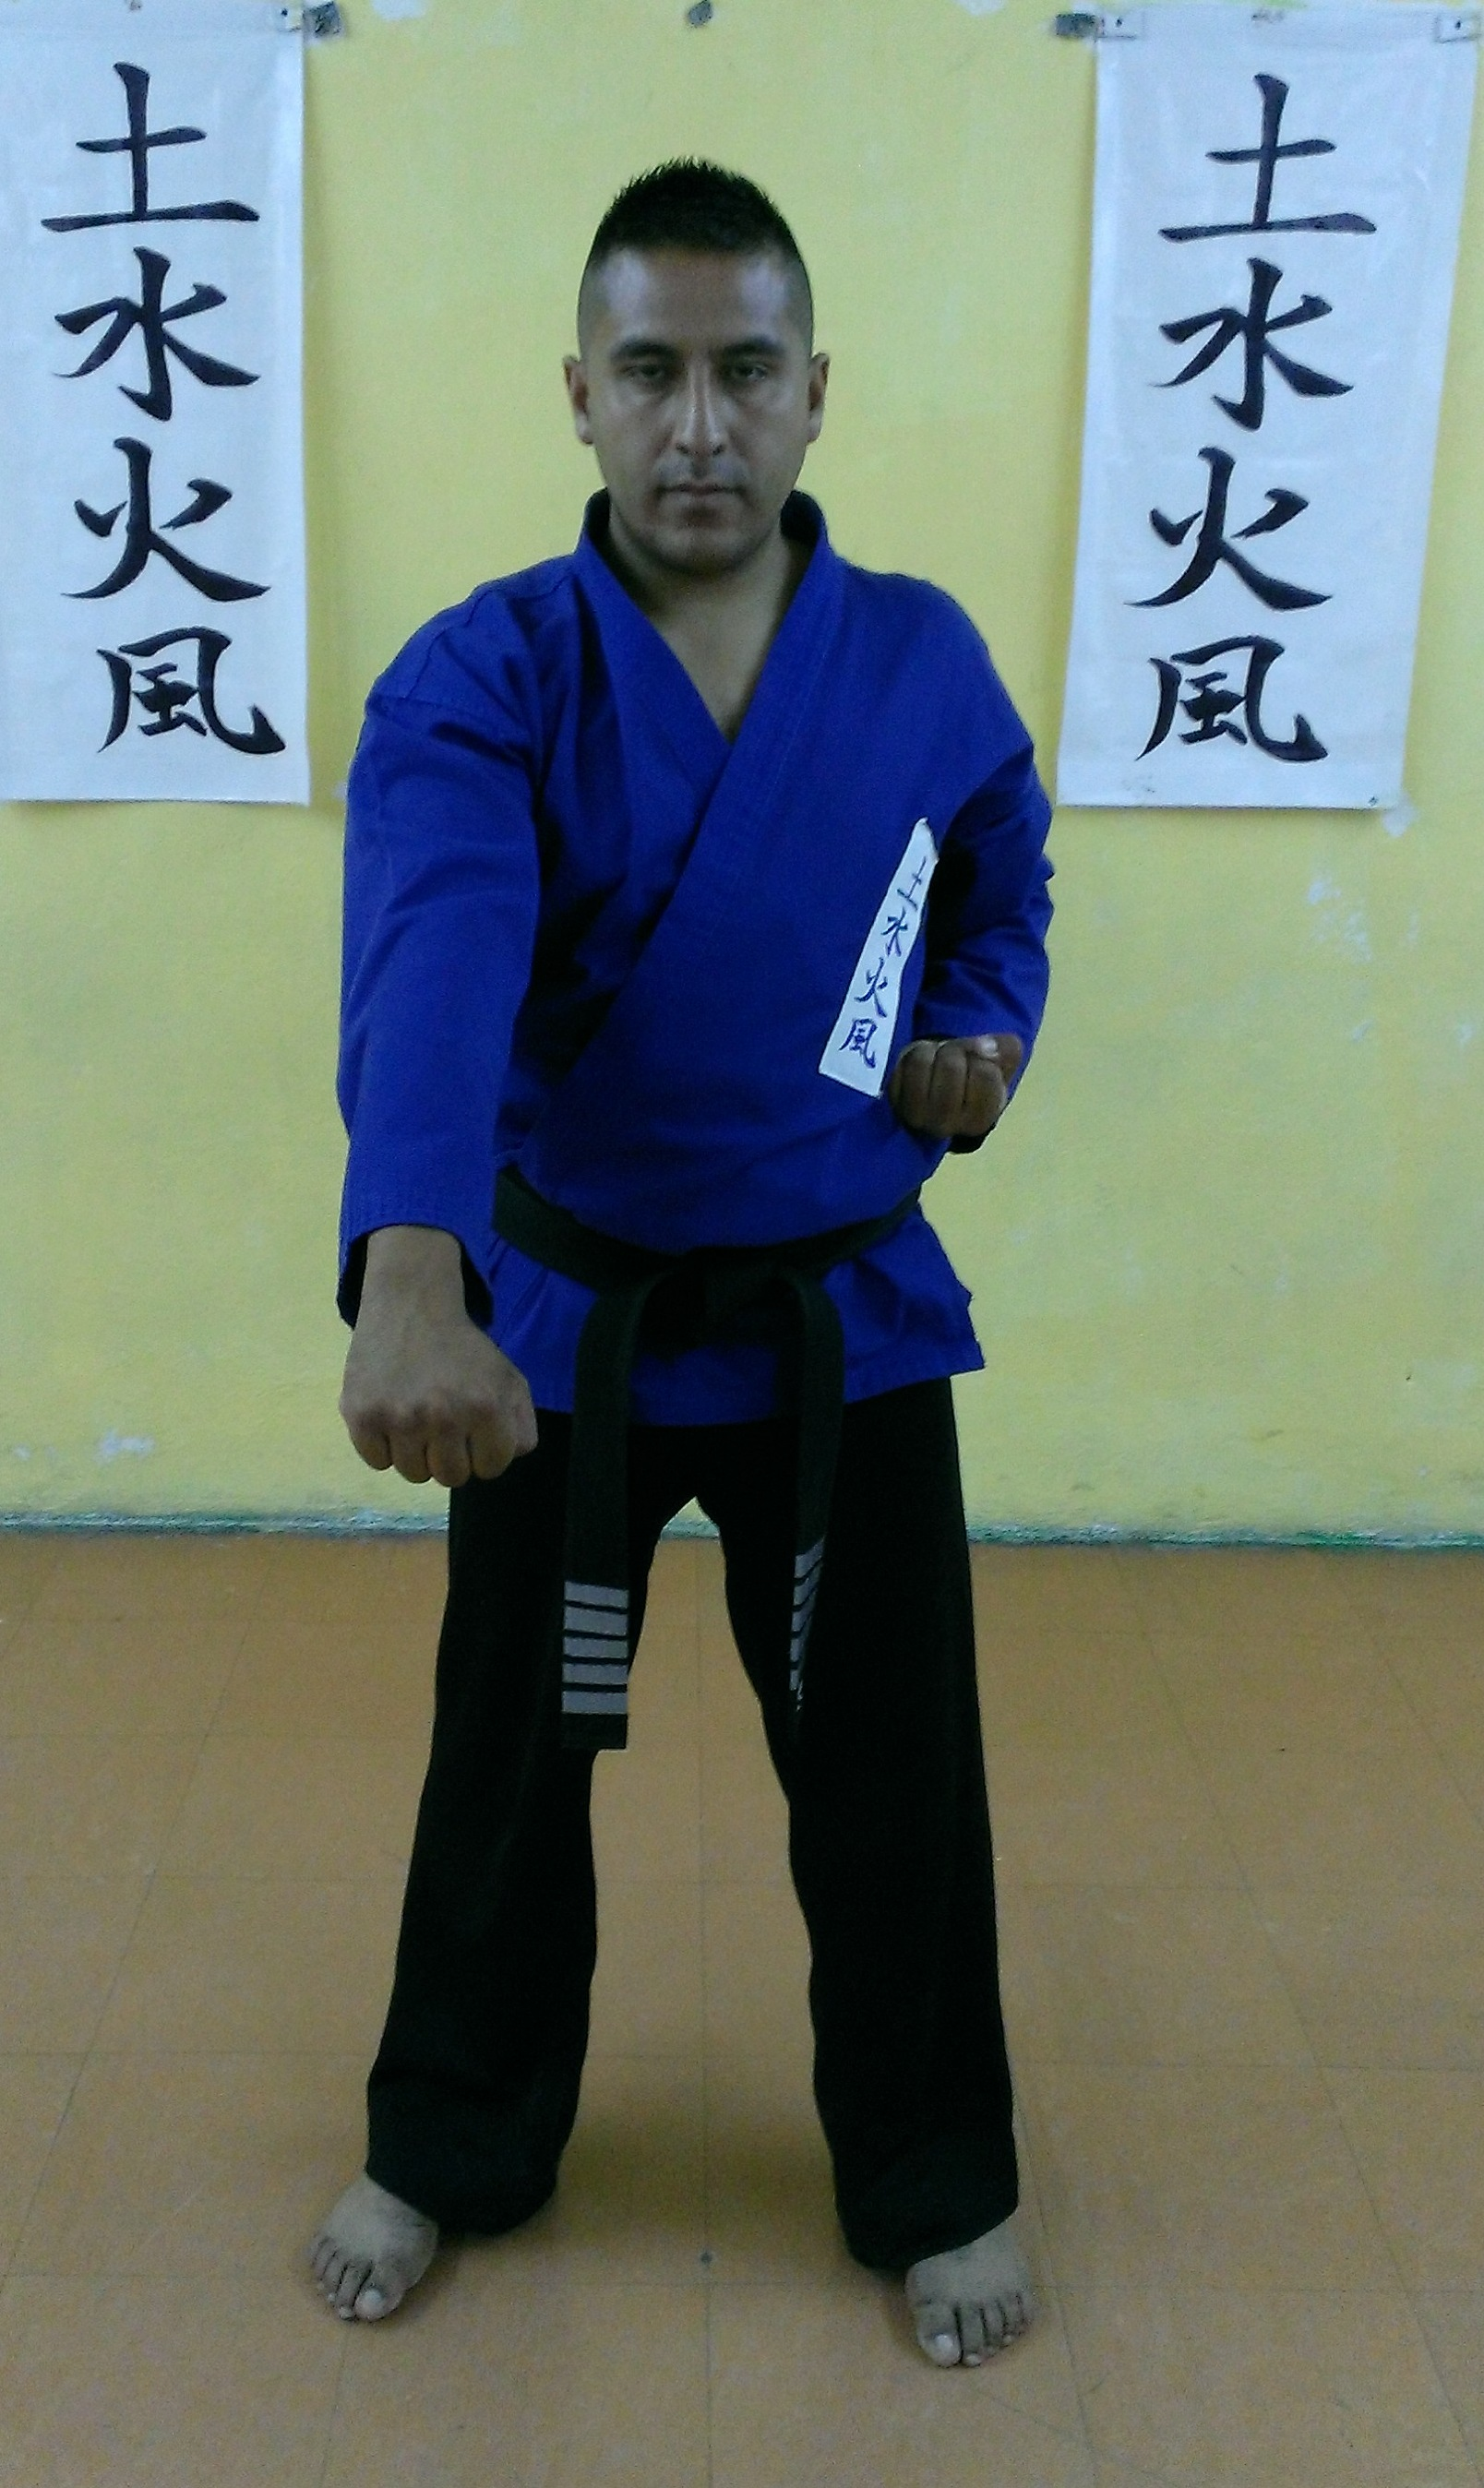
\includegraphics[width=5cm, height=8cm]{./Figuras/Tecnica/GedanBaraiUke_Frontal}}
	\subfloat[Defensa Gedan Barai Uke lateral]{
		\label{fig:GedanBaraiUke_Lateral}
		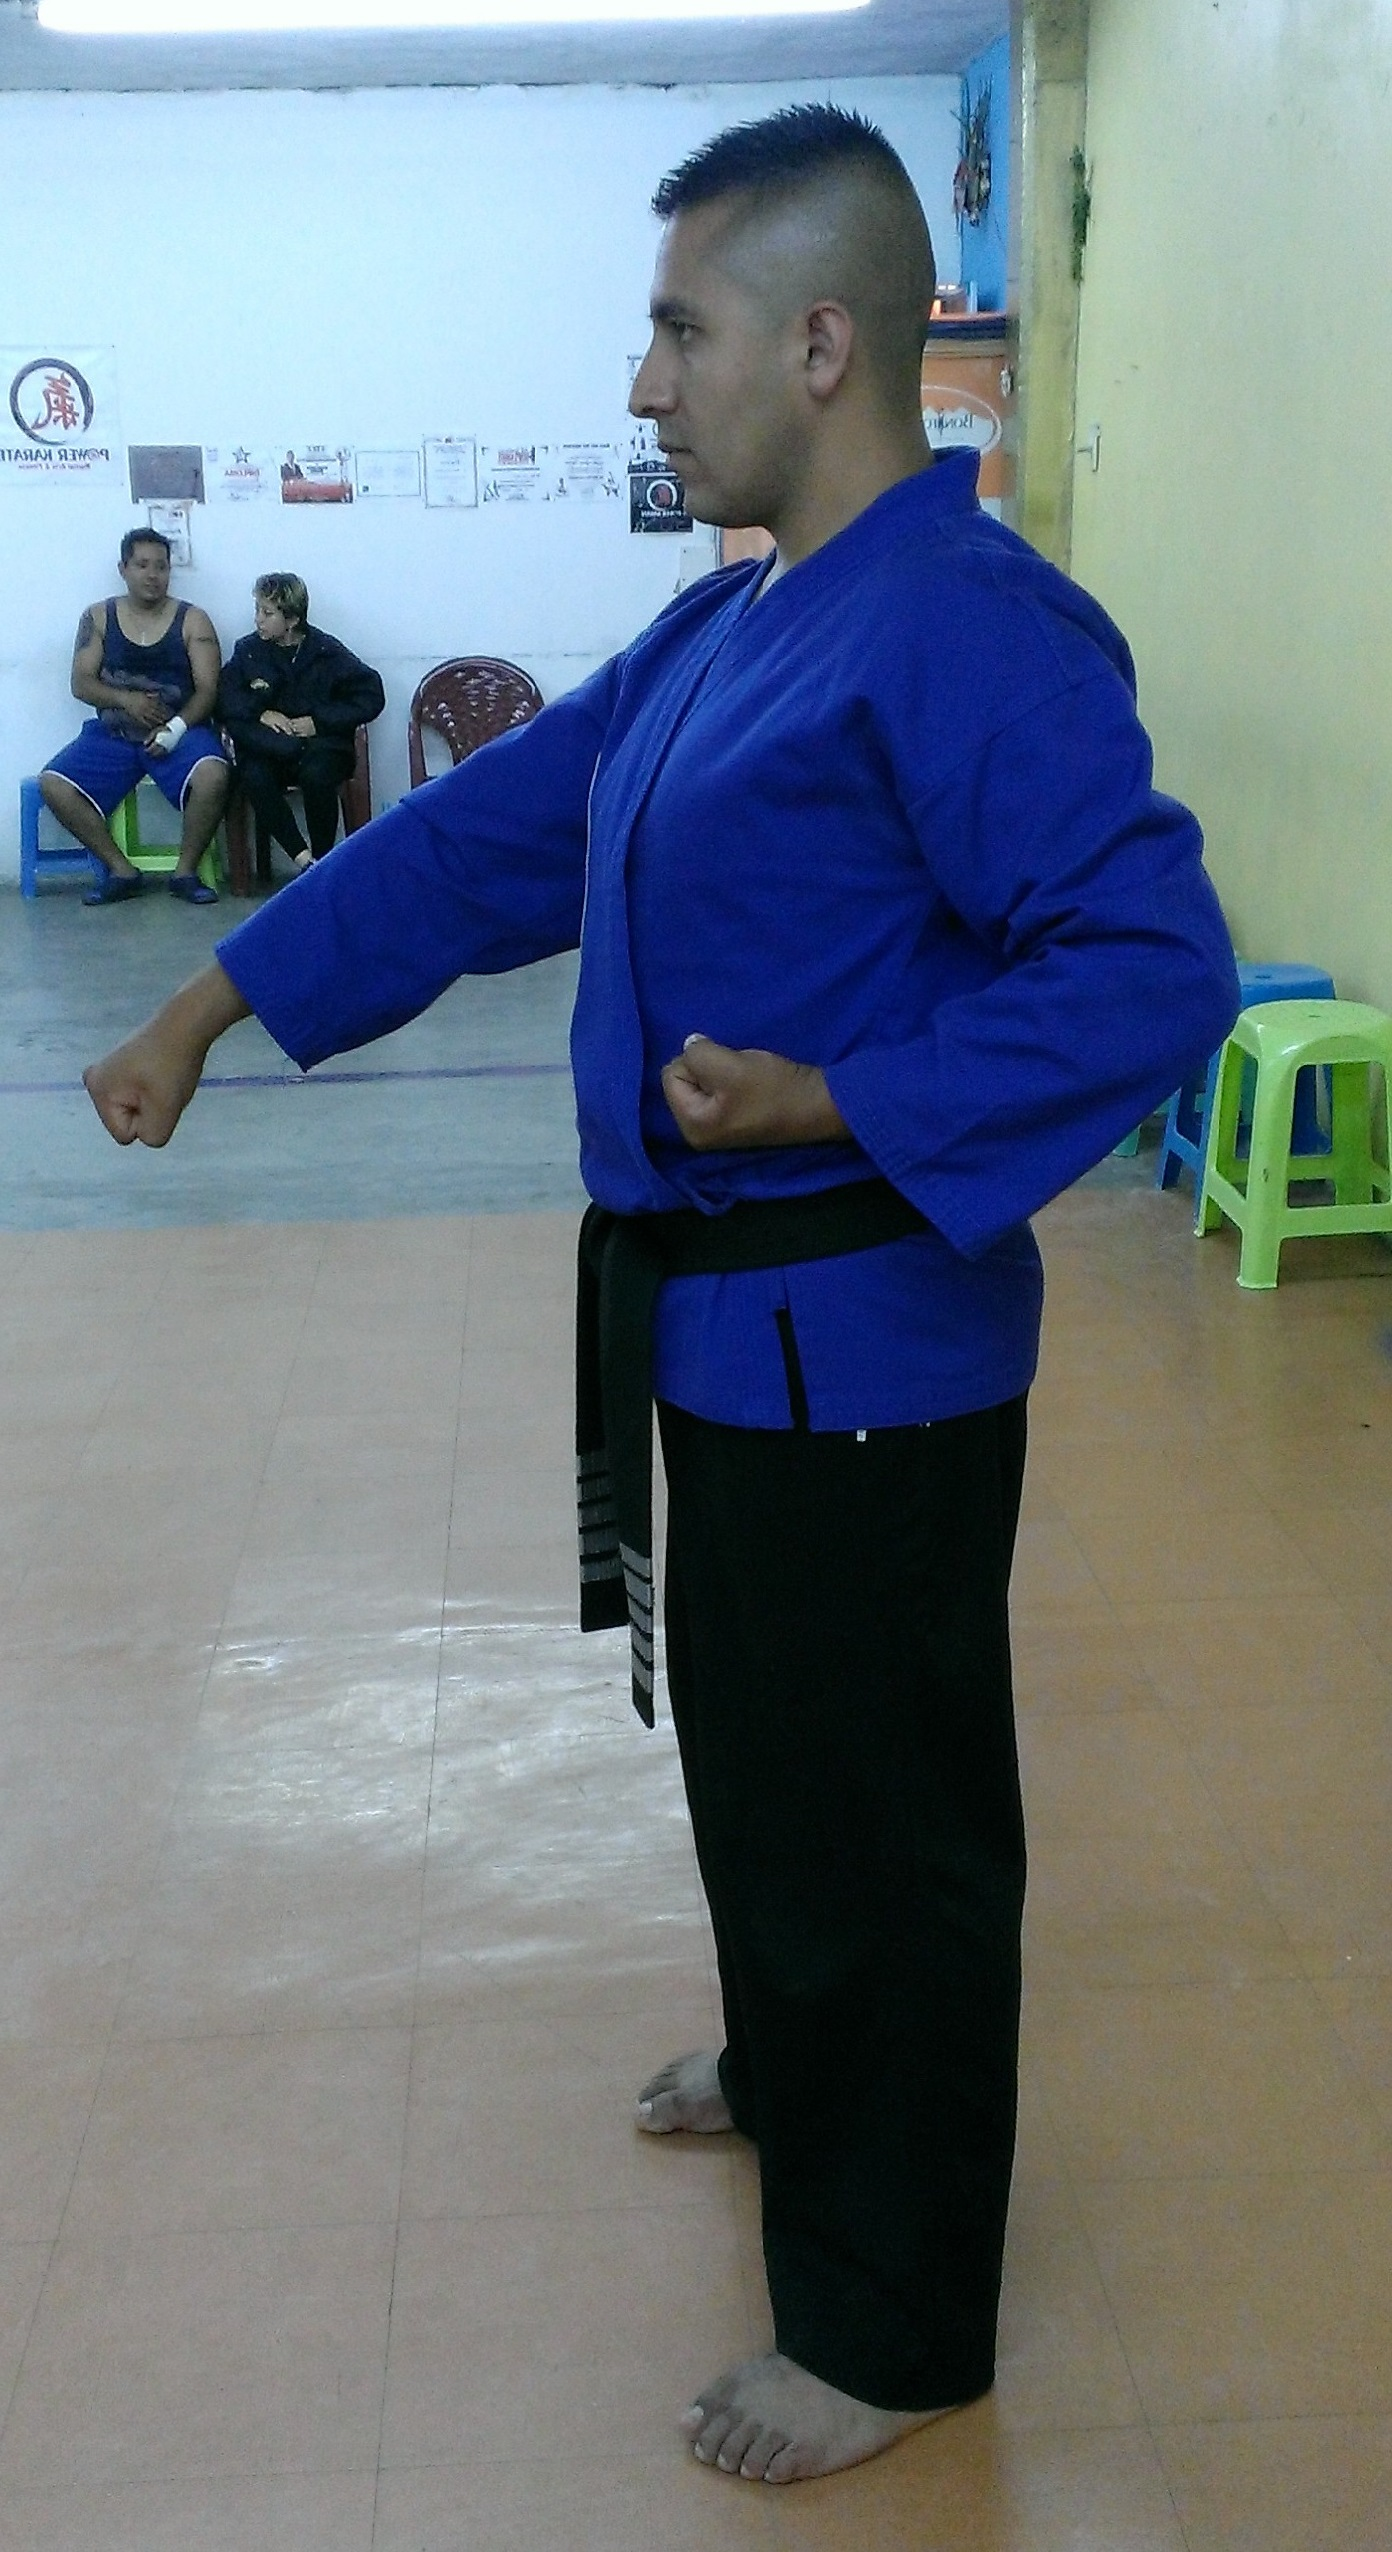
\includegraphics[width=5cm, height=8cm]{./Figuras/Tecnica/GedanBaraiUke_Lateral}}
	\caption{Defensa Gedan Barai Uke}
	\label{fig:Defensas1}
\end{figure}

\begin{figure}[H]
	\centering
	\subfloat[Defensa Shudan Soto Uke frontal]{
		\label{fig:ShudanSotoUke_Frontal}
		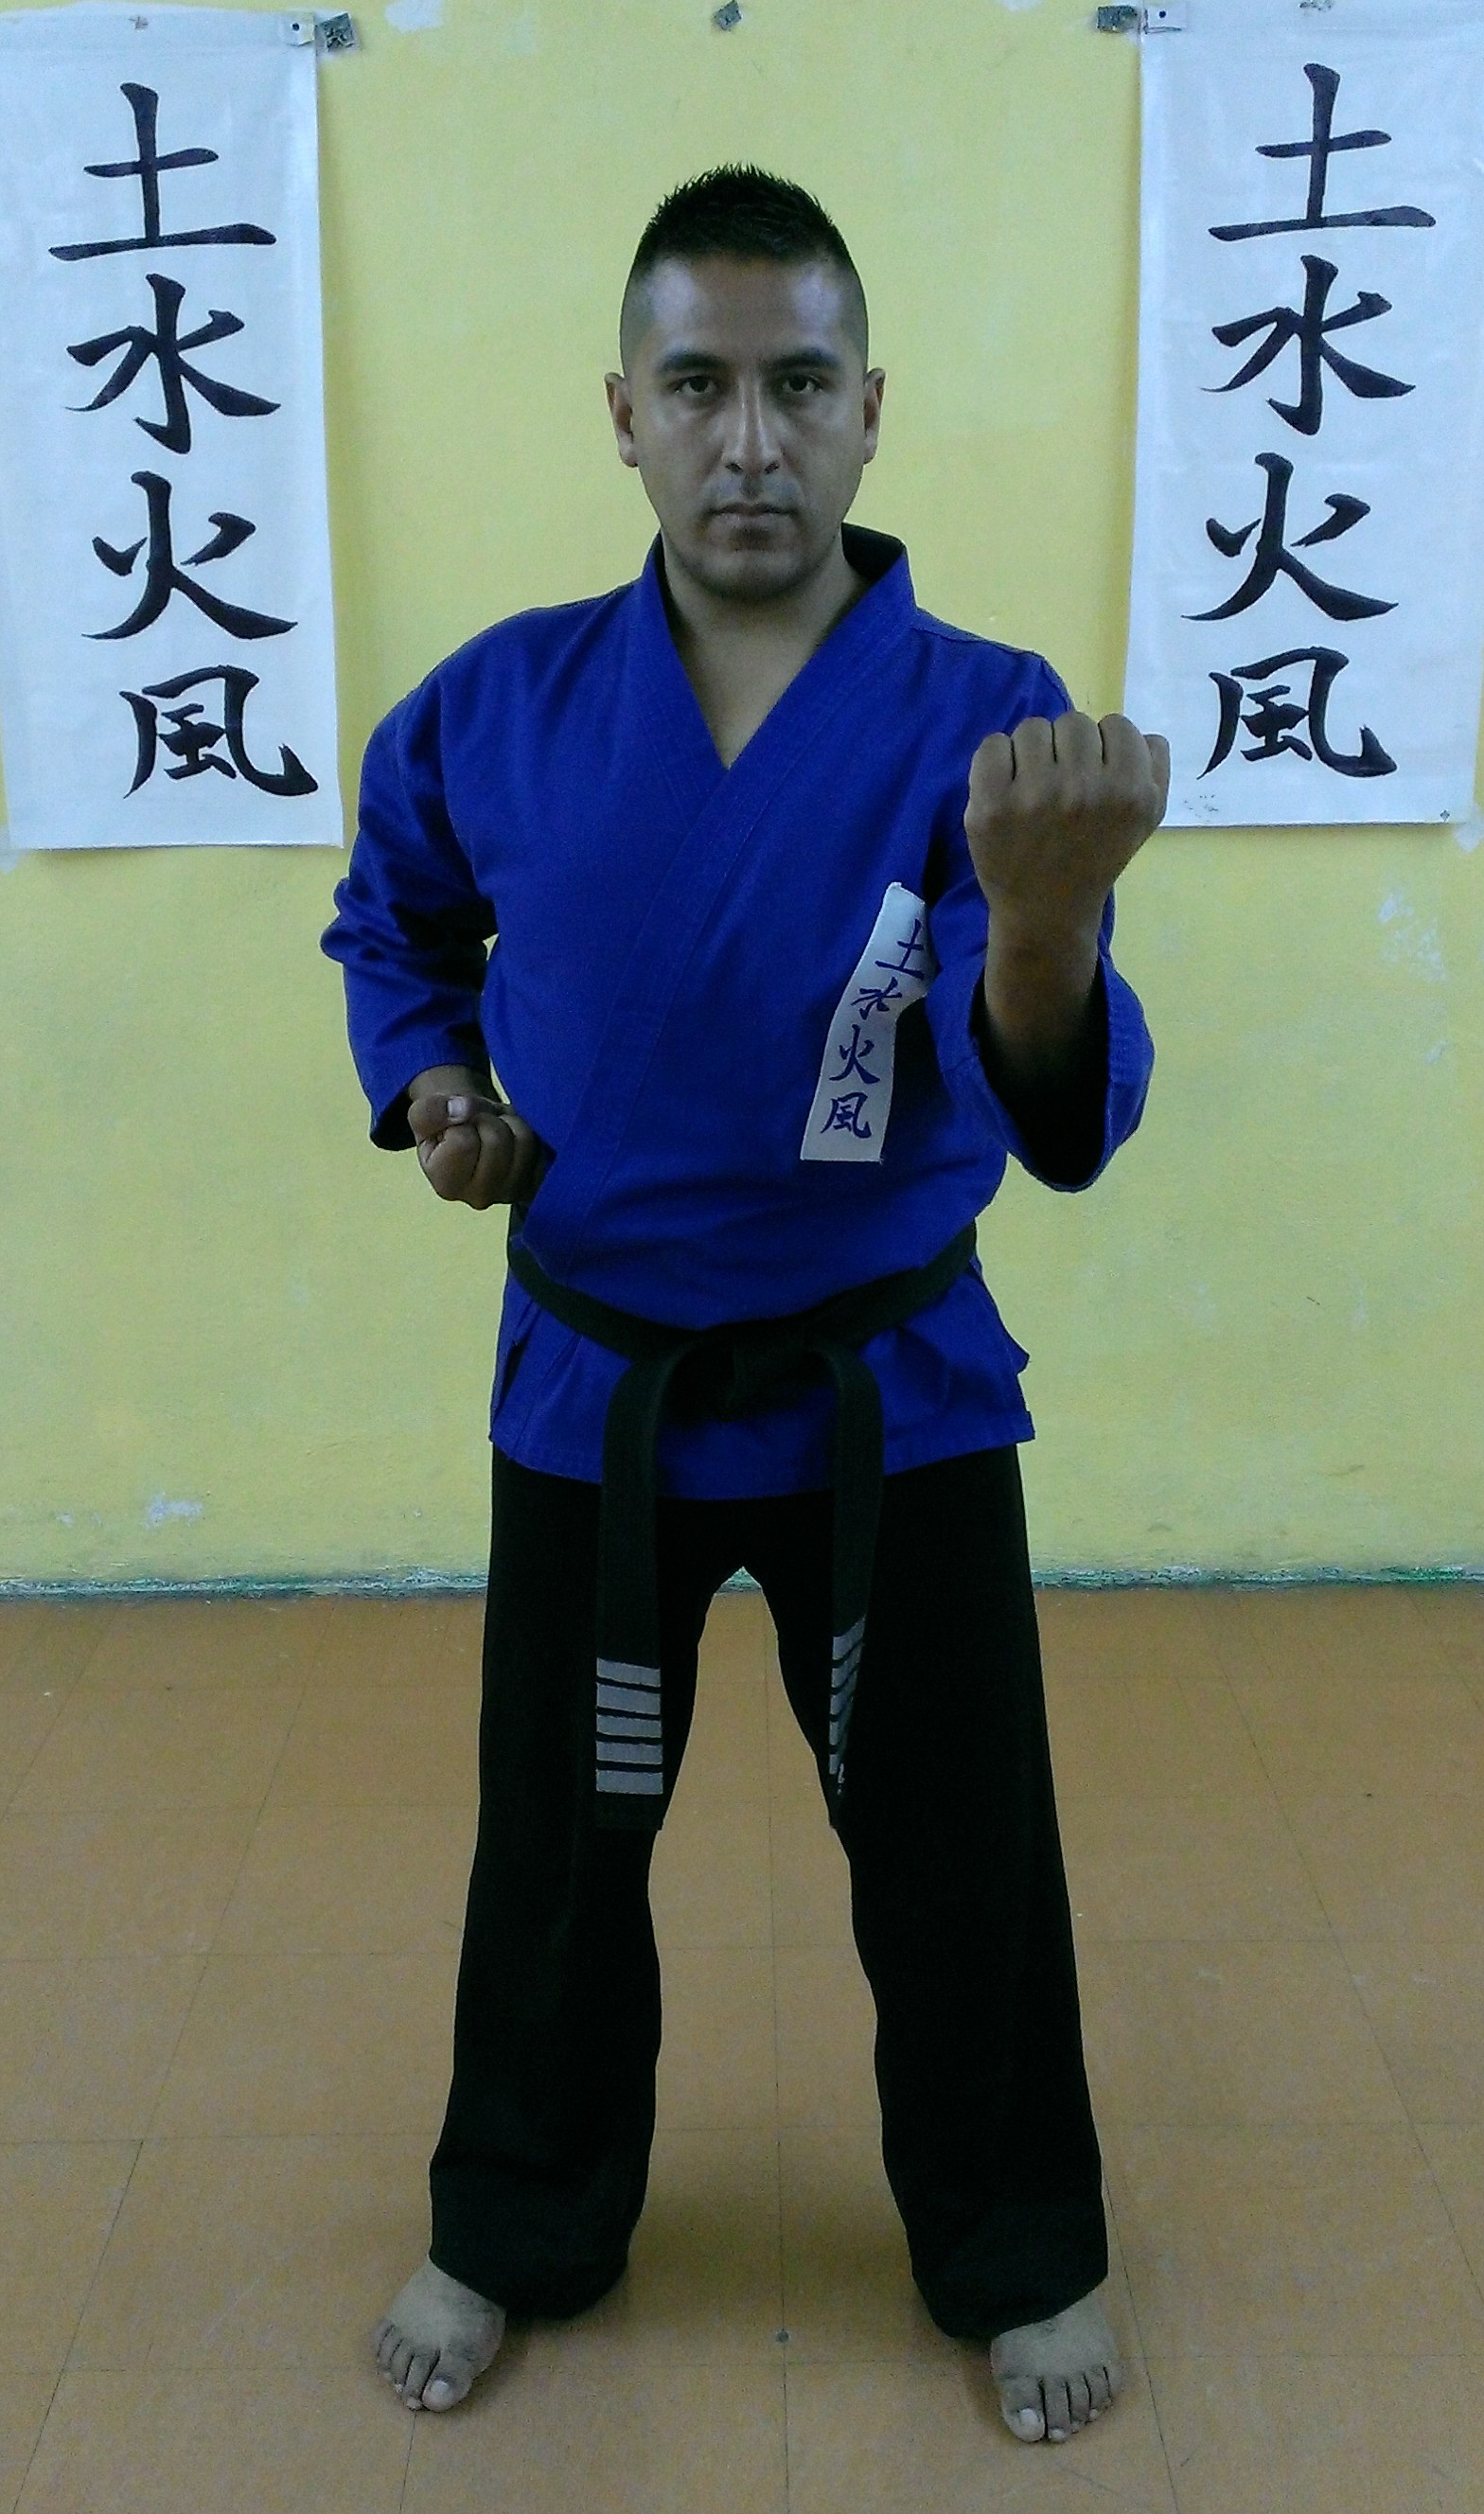
\includegraphics[width=5cm, height=8cm]{./Figuras/Tecnica/ShudanSotoUke_Frontal}}
	\subfloat[Defensa Shudan Soto Uke lateral]{
		\label{fig:ShudanSotoUke_Lateral}
		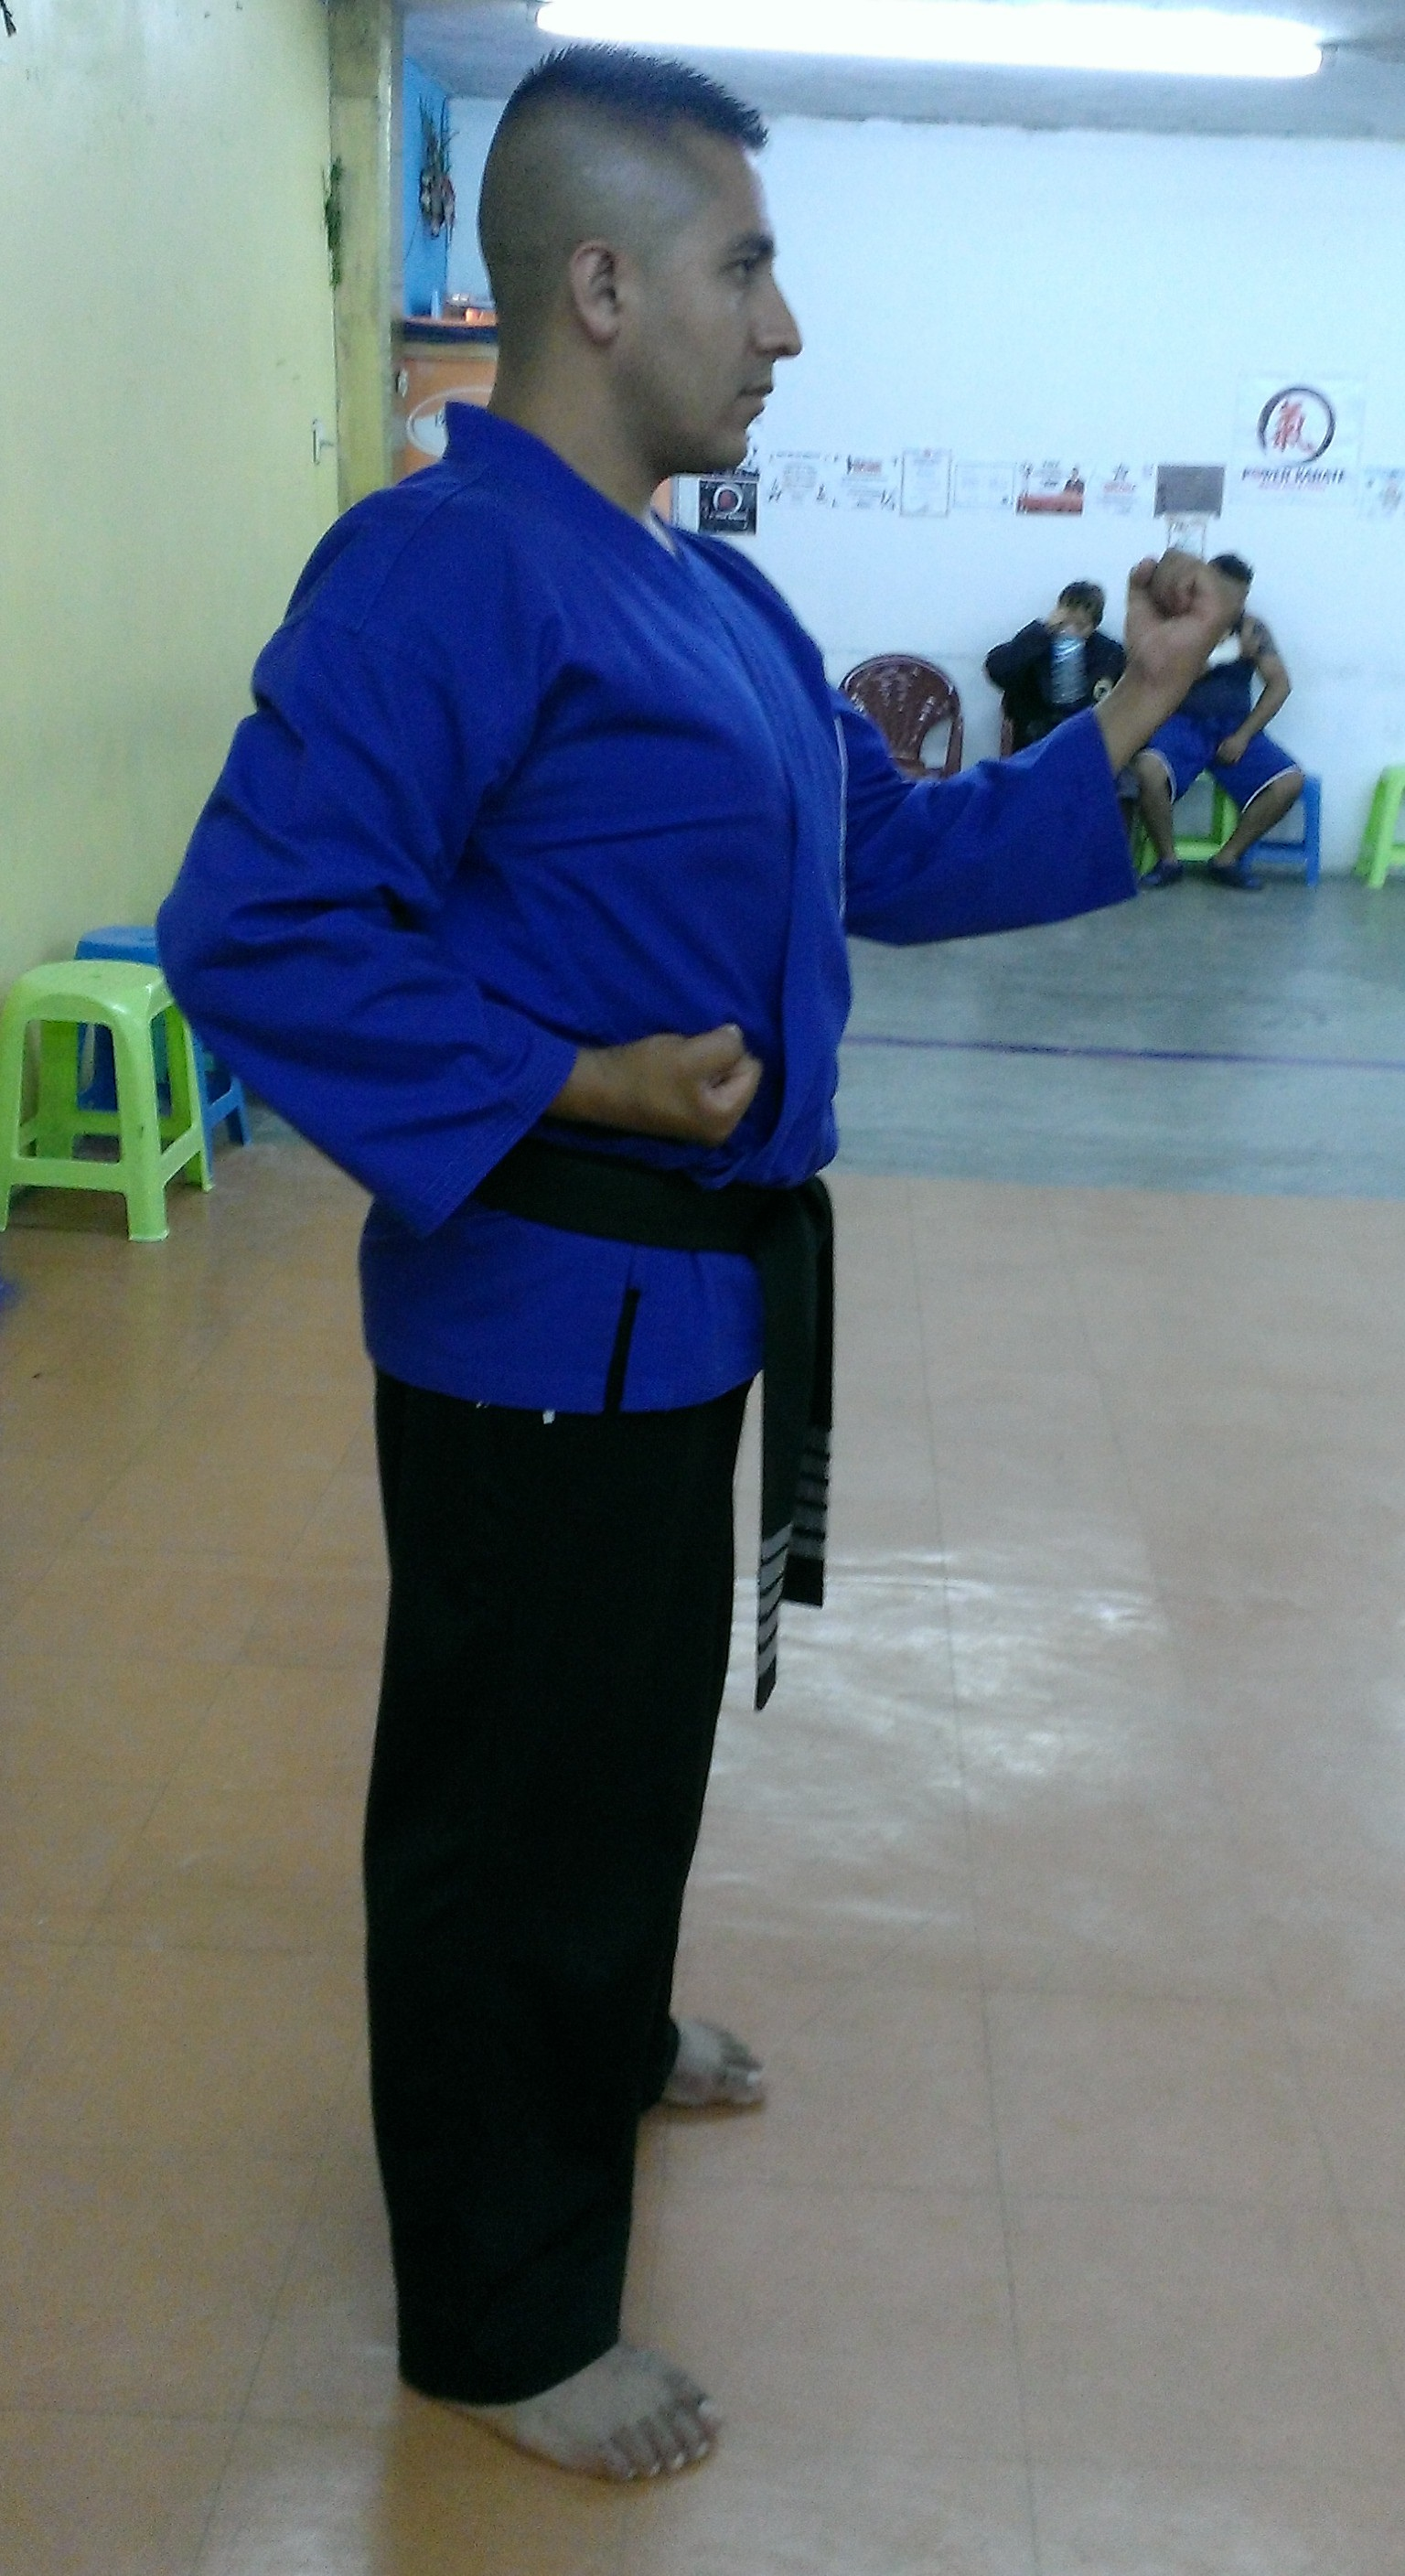
\includegraphics[width=5cm, height=8cm]{./Figuras/Tecnica/ShudanSotoUke_Lateral}}
	\caption{Defensa Shudan Soto Uke}
	\label{fig:Defensas2}
\end{figure}

\begin{figure}[H]
	\centering
	\subfloat[Defensa Yodan Age Uke frontal]{
		\label{fig:YodanAgeUke_Frontal}
		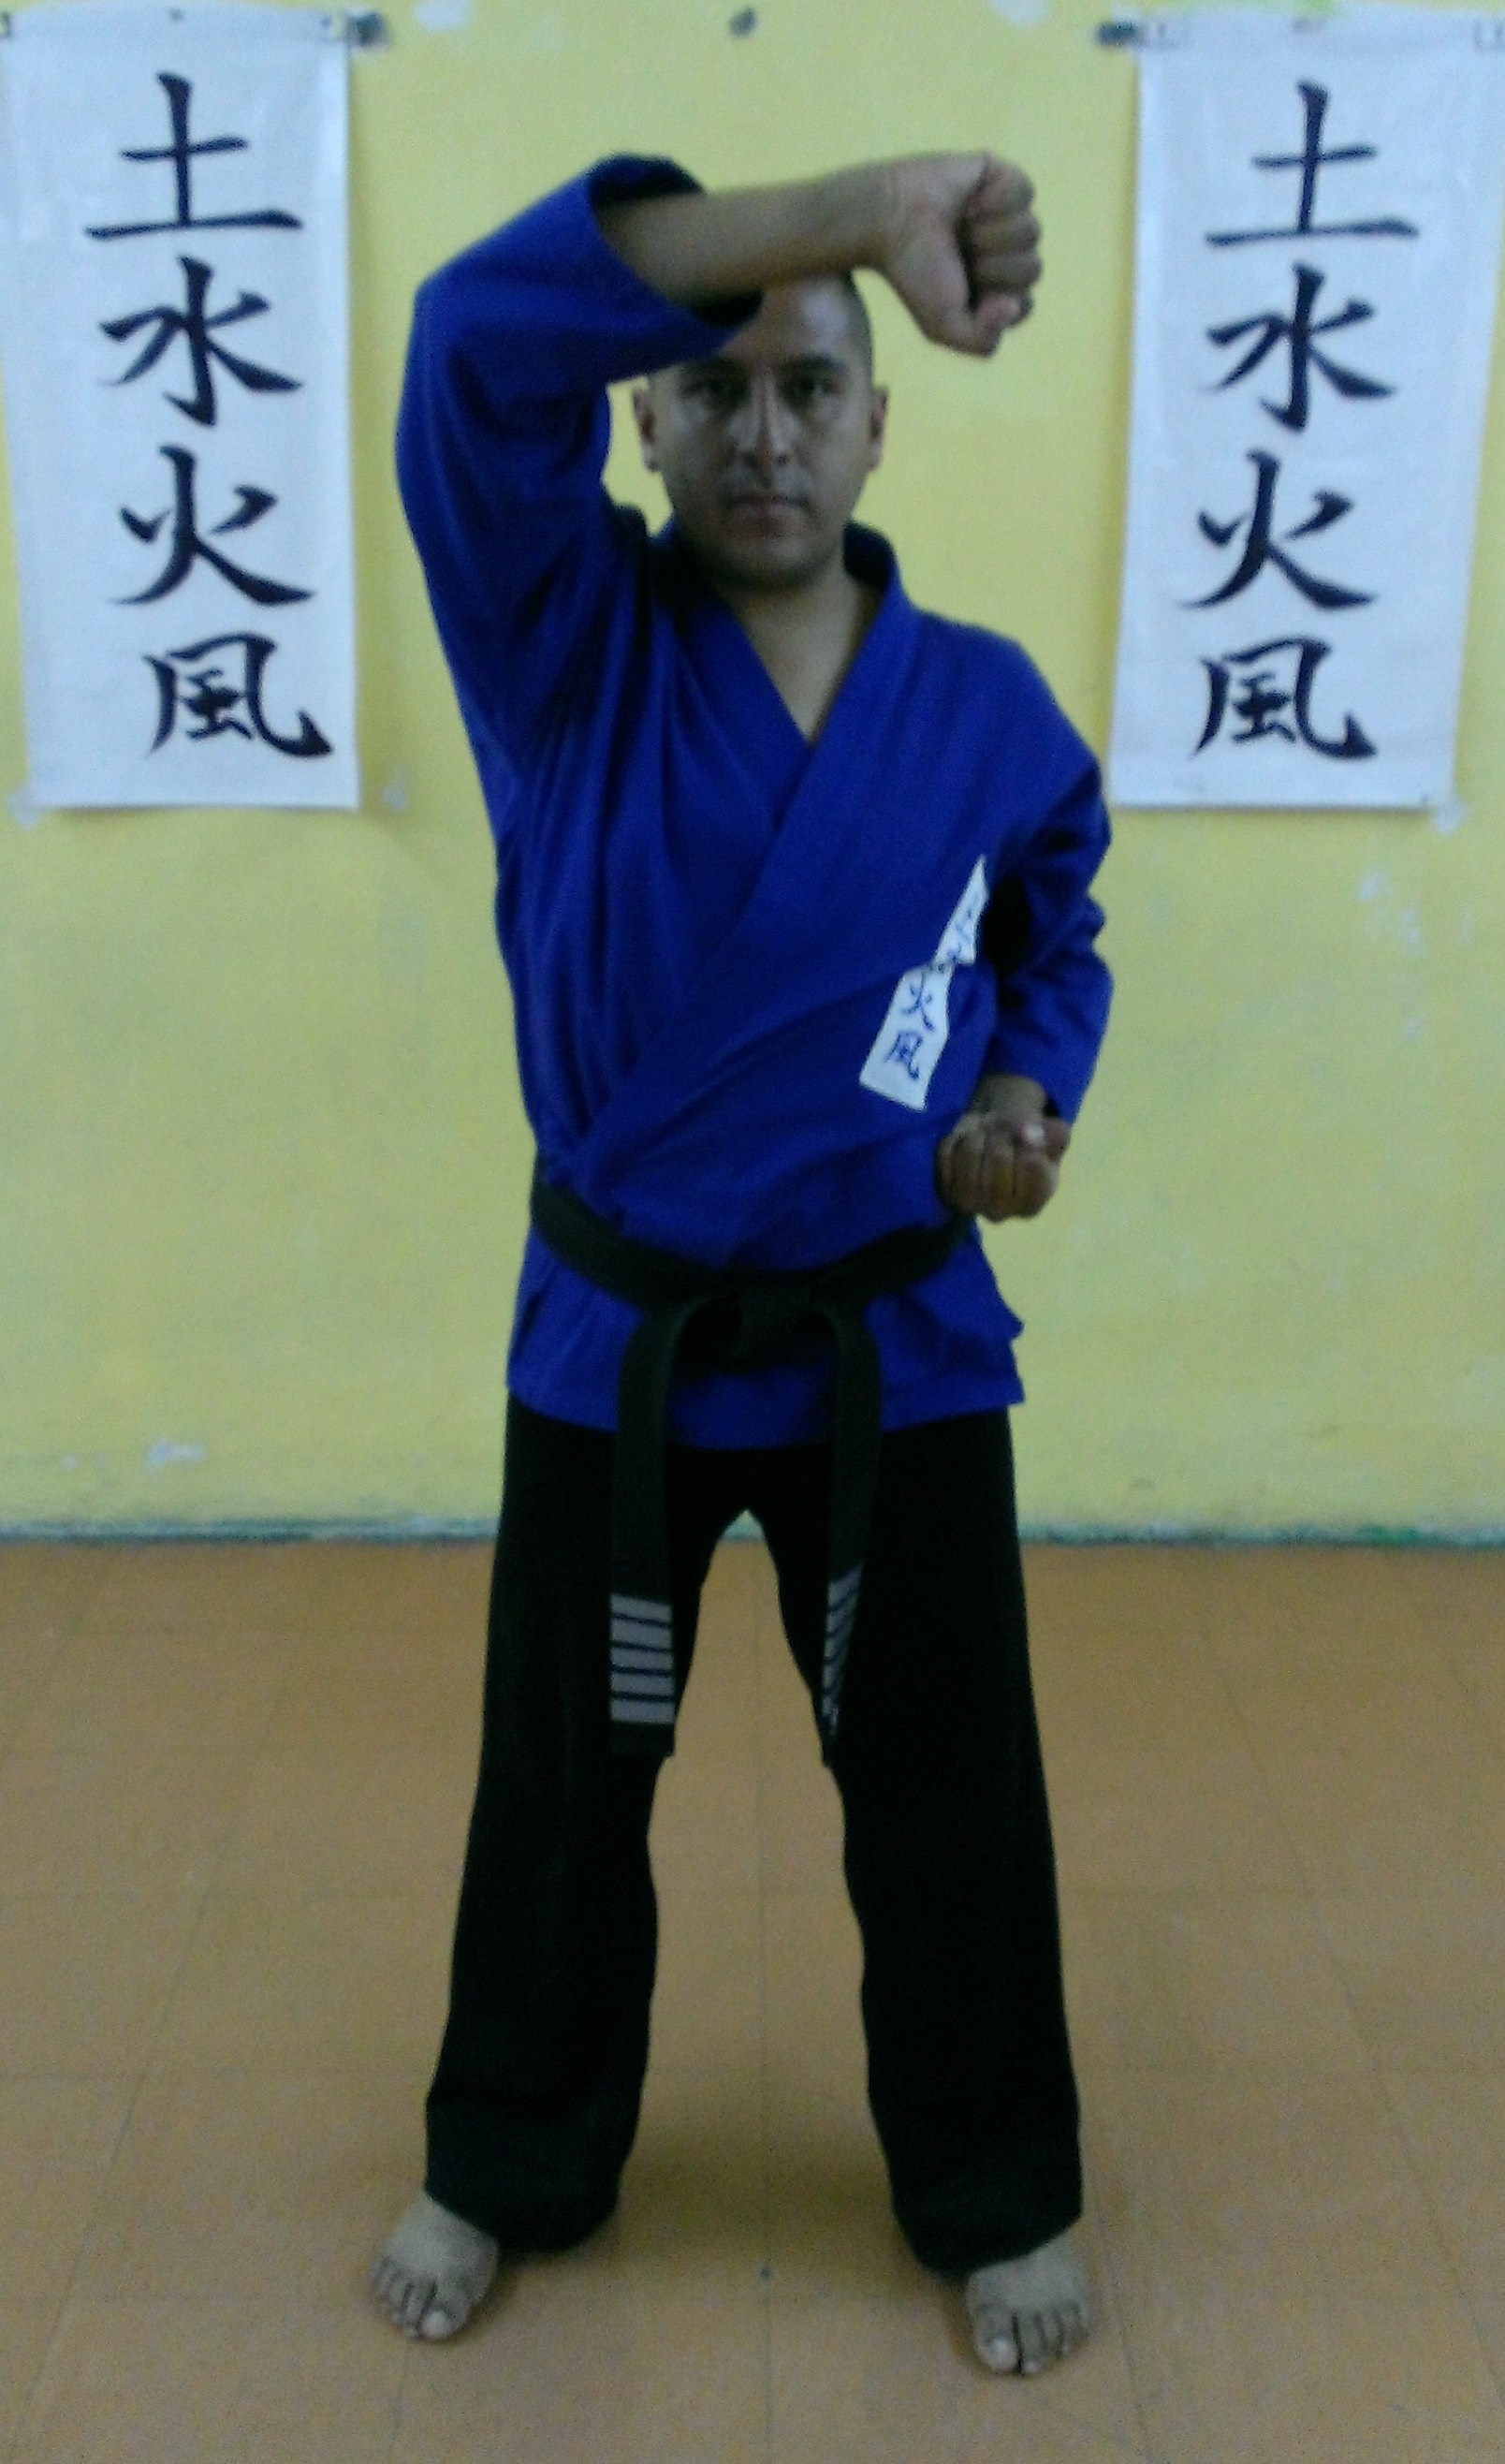
\includegraphics[width=5cm, height=8cm]{./Figuras/Tecnica/YodanAgeUke_Frontal}}
	\subfloat[Defensa Yodan Age Uke lateral]{
		\label{fig:YodanAgeUke_Lateral}
		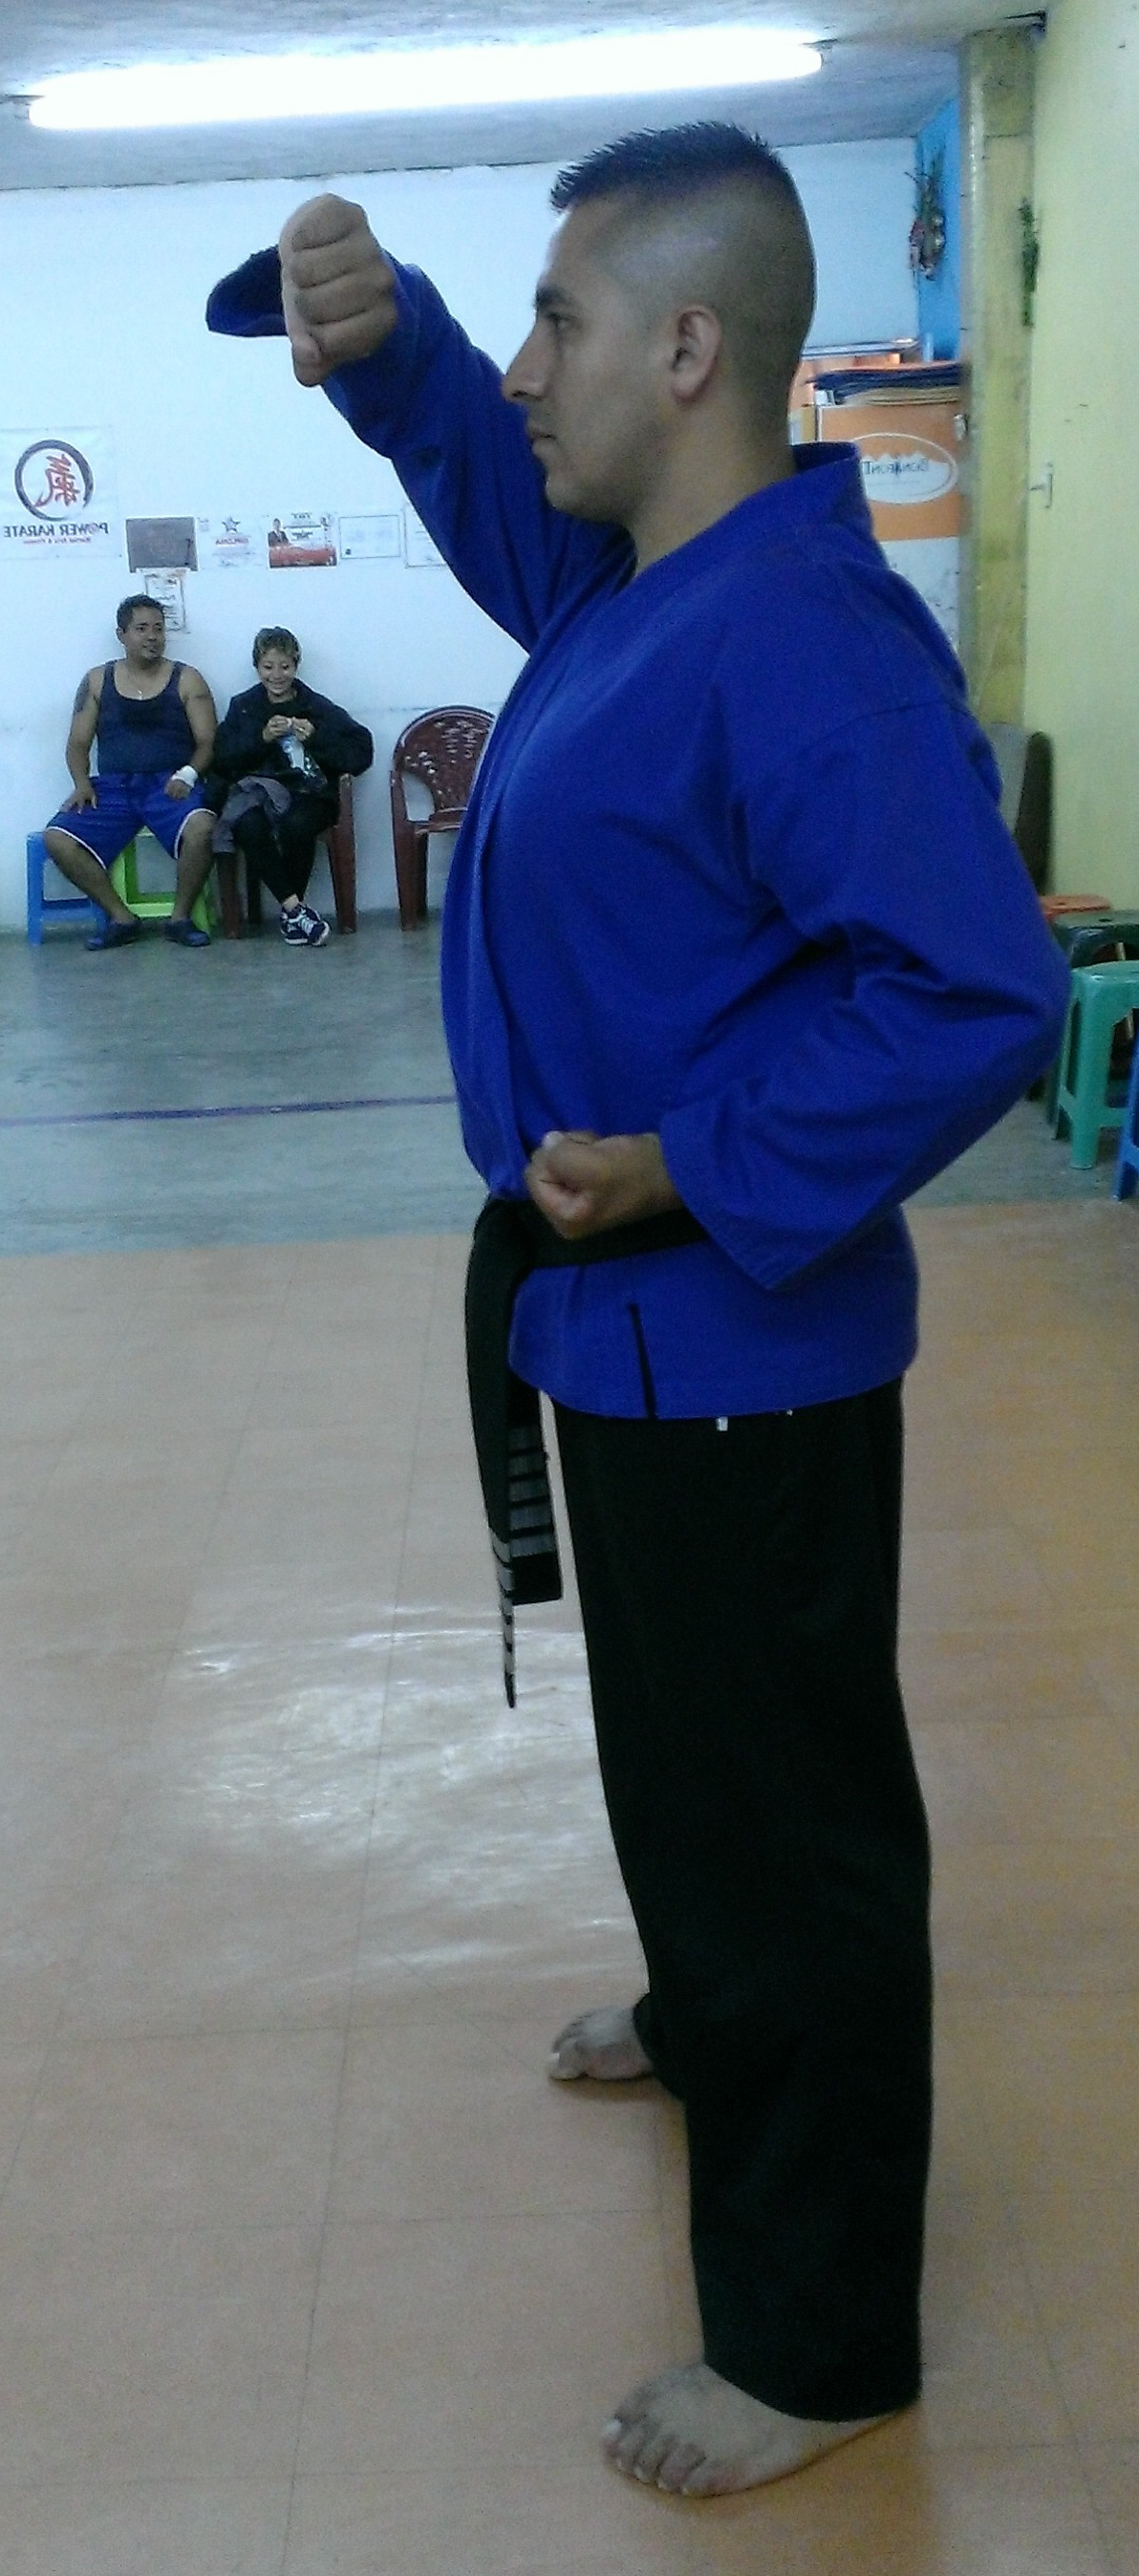
\includegraphics[width=4.5cm, height=8cm]{./Figuras/Tecnica/YodanAgeUke_Lateral}}
	\caption{Defensa Yodan Age Uke}
	\label{fig:Defensas3}
\end{figure}

\begin{figure}[H]
	\centering
	\subfloat[Ataque con brazo Seiken Tsuki frontal]{
		\label{fig:SeikenTsuki_Frontal}
		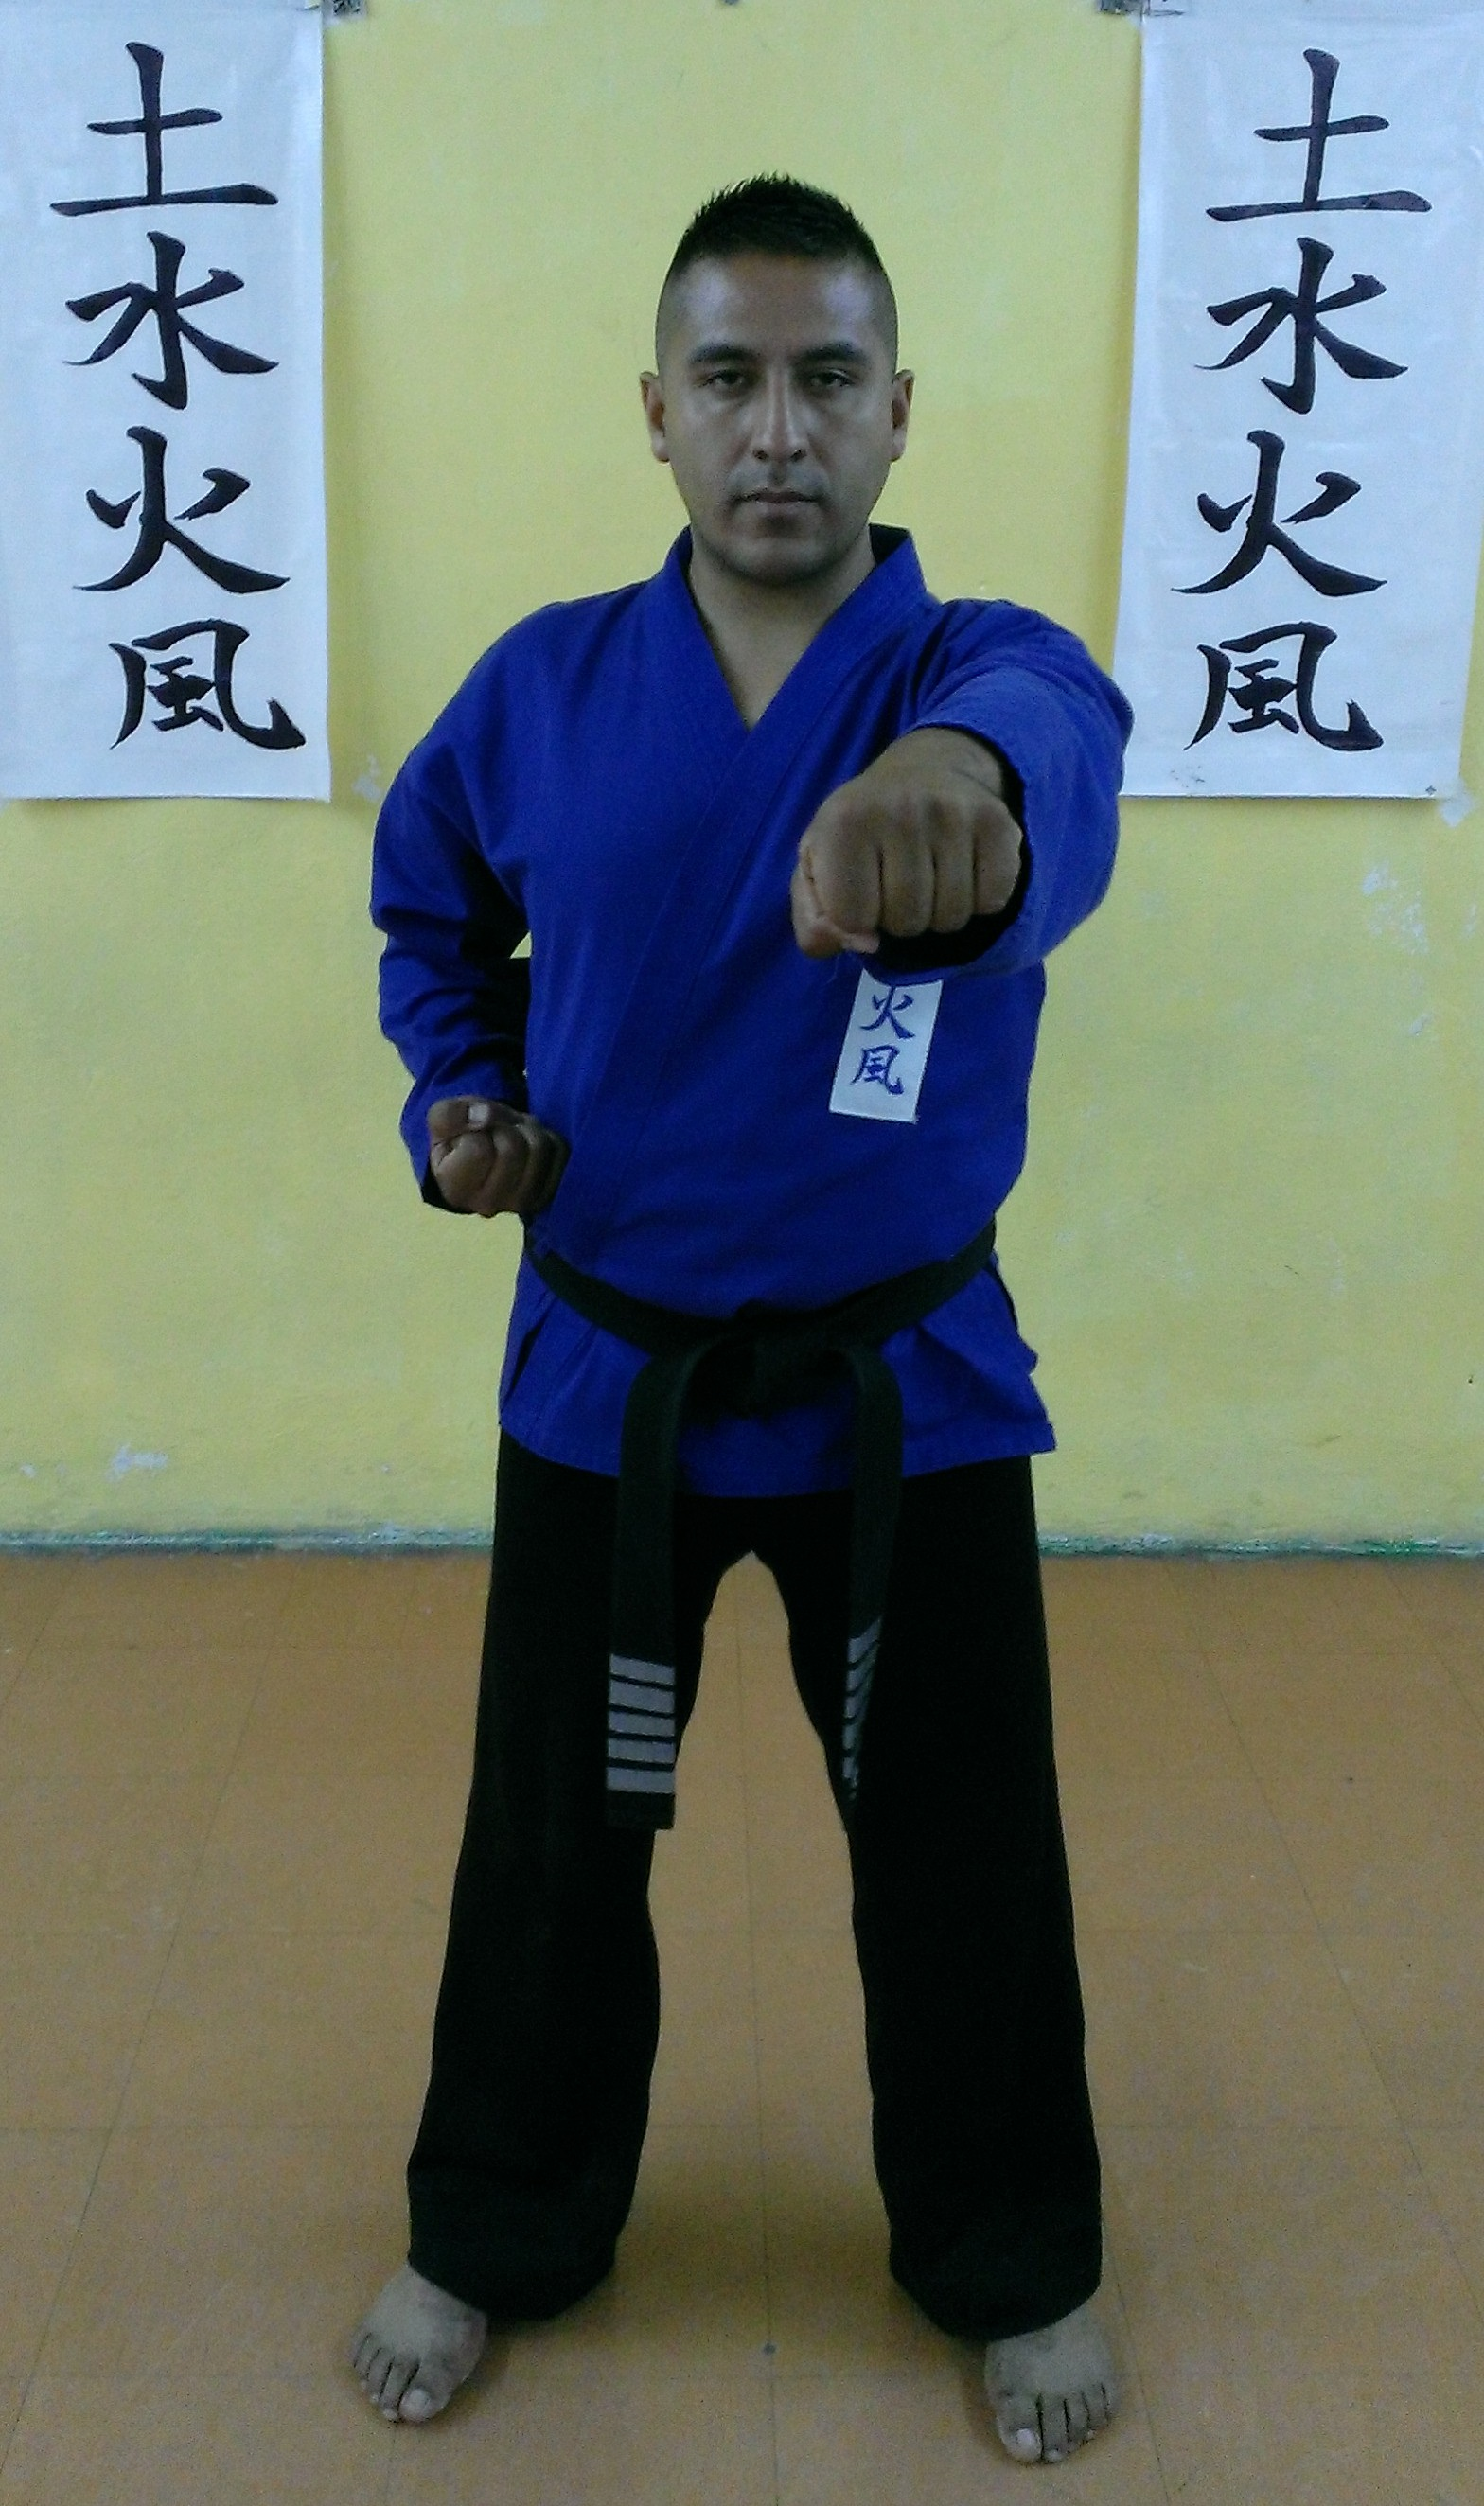
\includegraphics[width=5cm, height=8cm]{./Figuras/Tecnica/SeikenTsuki_Frontal}}
	\subfloat[Ataque con brazo Seiken Tsuki lateral]{
		\label{fig:SeikenTsuki_Lateral}
		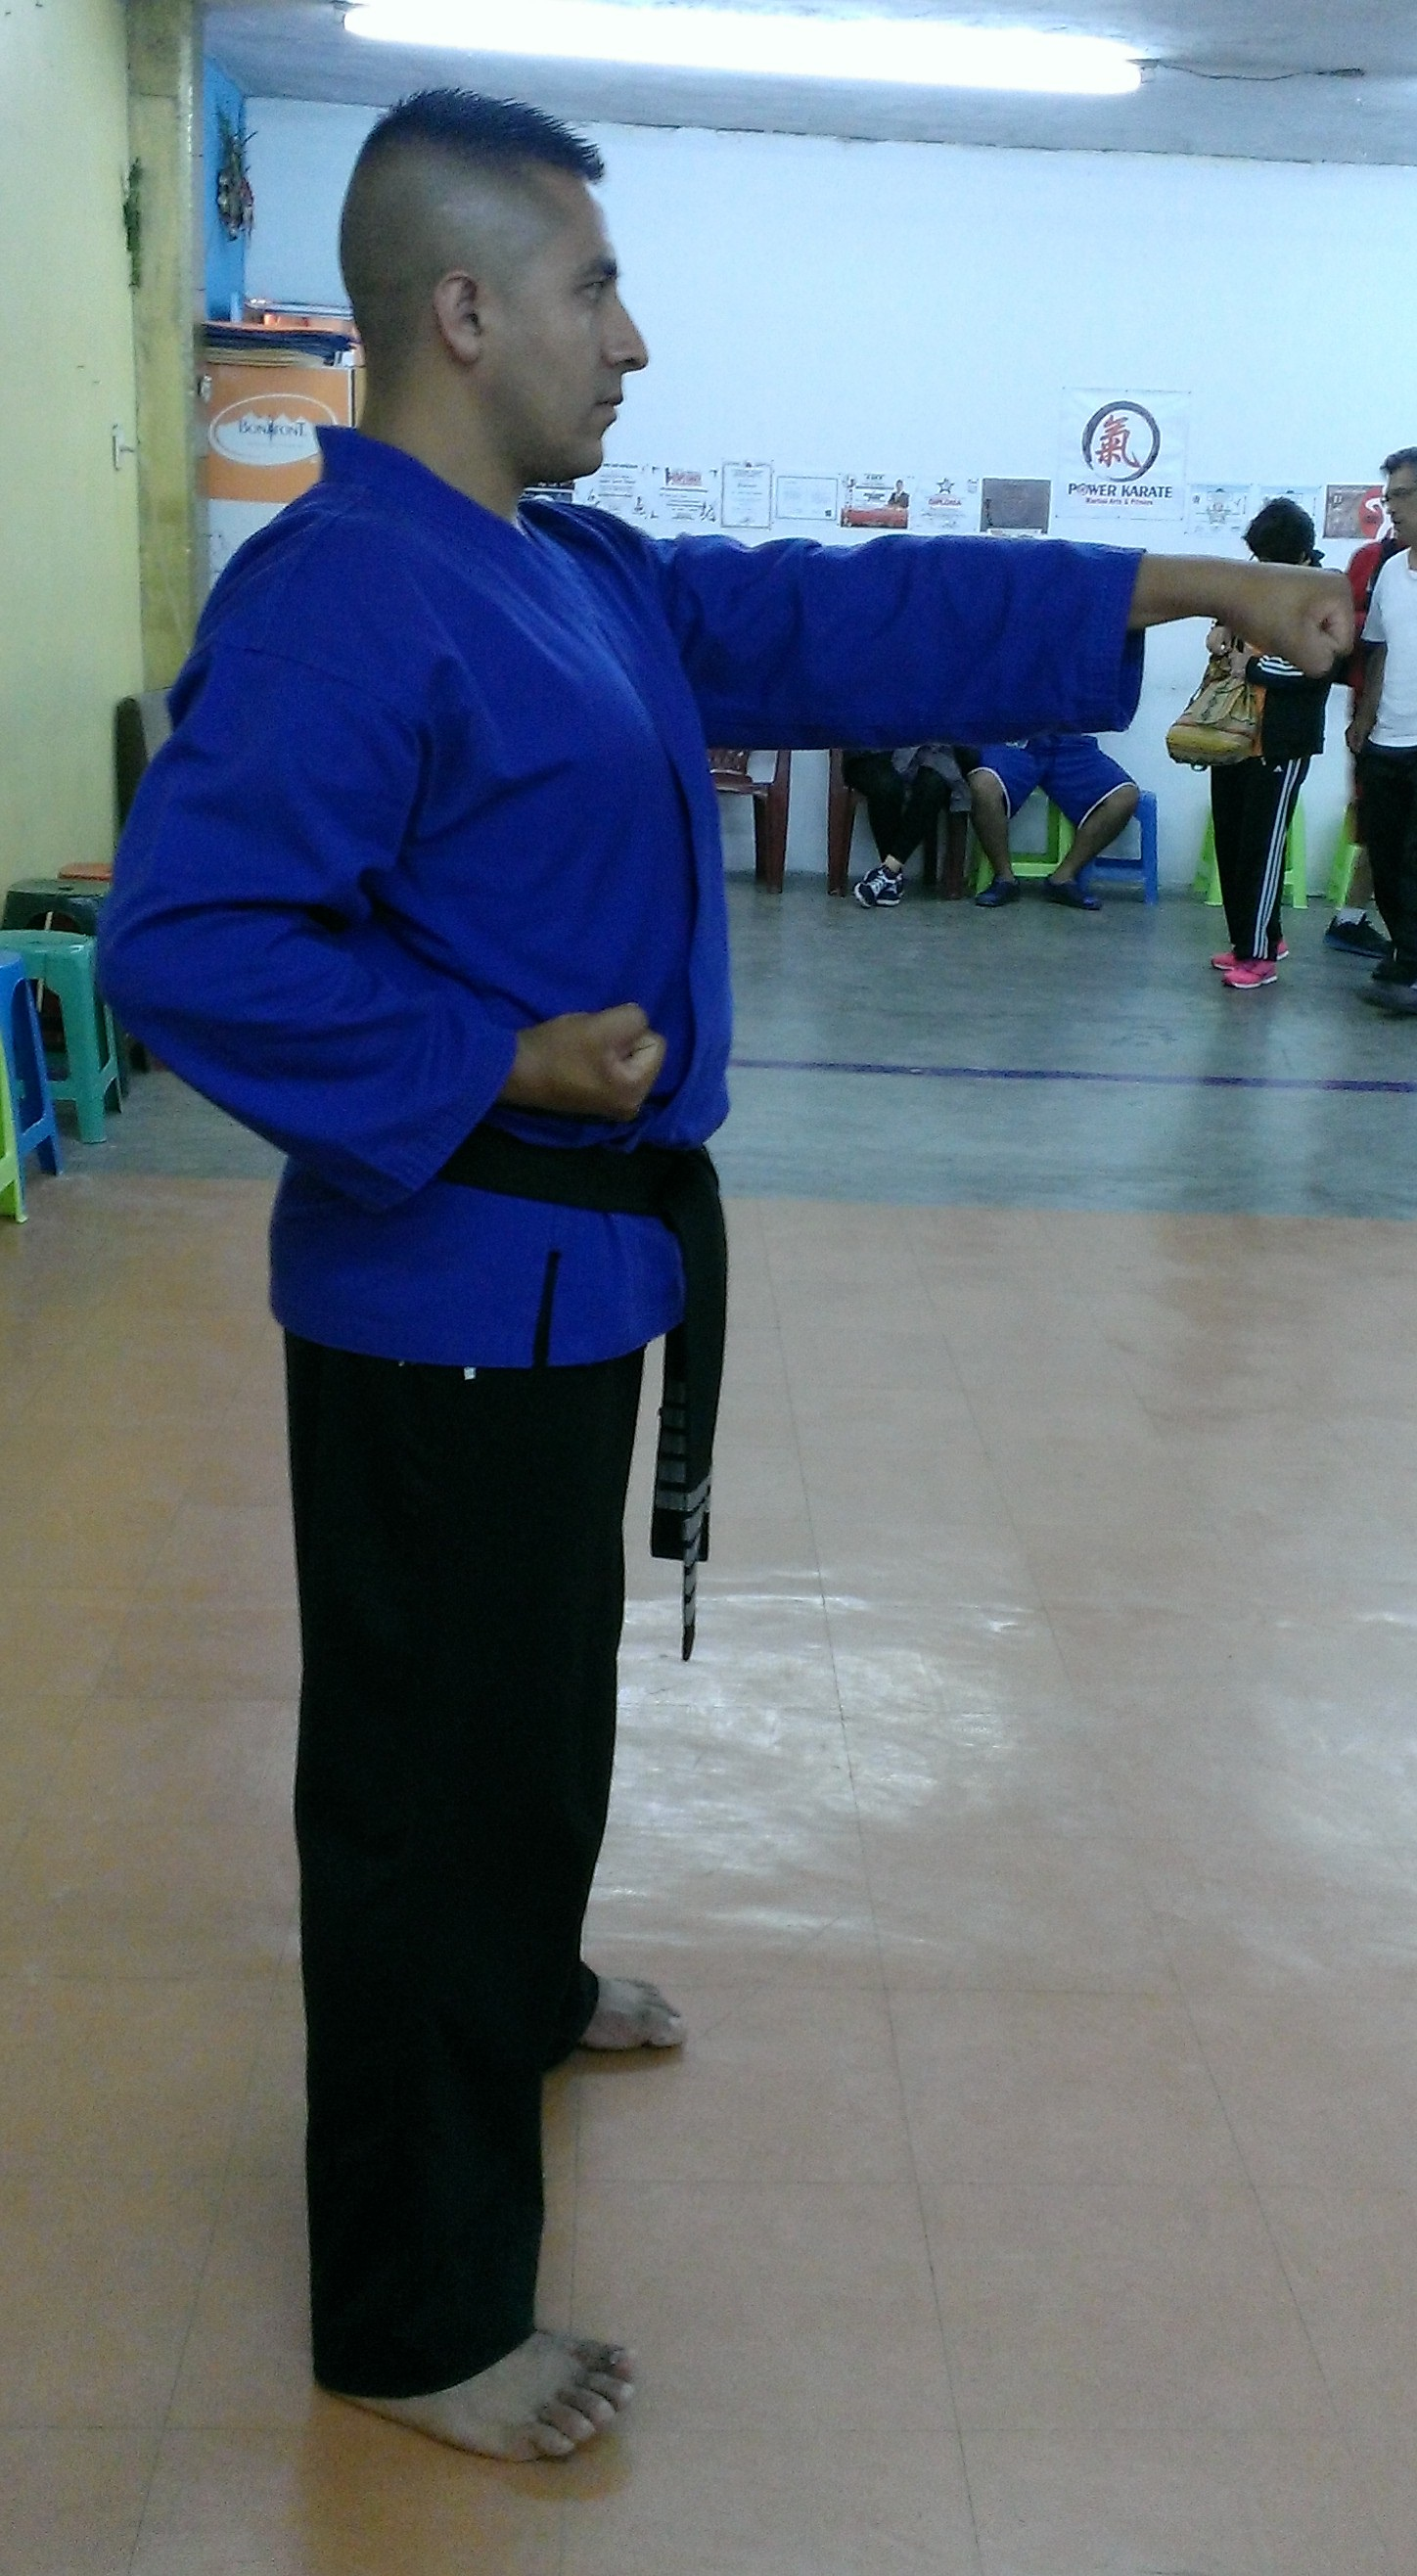
\includegraphics[width=5cm, height=8cm]{./Figuras/Tecnica/SeikenTsuki_Lateral}}
	\caption{Ataque con brazo Seiken Tsuki}
	\label{fig:Ataques1}
\end{figure}

\begin{figure}[H]
	\centering
	\subfloat[Ataque con pierna Mae Geri frontal]{
		\label{fig:MaeGeri_Frontal}
		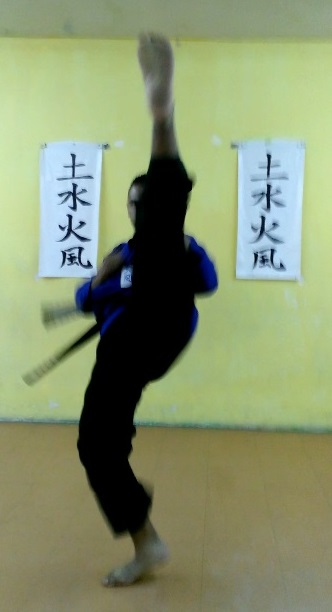
\includegraphics[width=5.5cm, height=8cm]{./Figuras/Tecnica/MaeGeri_Frontal}}
	\subfloat[Ataque con pierna Mae Geri lateral]{
		\label{fig:MaeGeri_Lateral}
		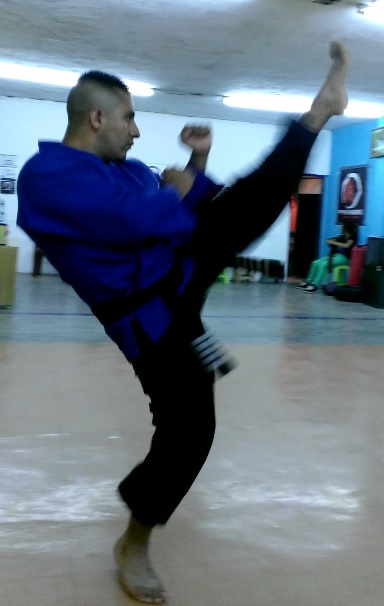
\includegraphics[width=5cm, height=8cm]{./Figuras/Tecnica/MaeGeri_Lateral}}
	\caption{Ataque con pierna Mae Geri}
	\label{fig:Ataques2}
\end{figure}

\clearpage
%-----------------------------------------------------------------------------
\subsubsection{Descripción de movimientos}
La siguiente tabla \ref{tab:DMT} \nameref{tab:DMT} muestra la descripción de los movimientos de técnica, clasificando el tipo de movimiento al que pertenece (posiciones, defensas o ataques).

\begin{table}[H]
\centering
\begin{tabular}{| p{4 cm} | p{2 cm} | p{9 cm} |}
\hline
\rowcolor[rgb]{0.529412, 0.807843, 0.980392} {\textbf{Nombre}} & {\textbf{Tipo}} & {\textbf{Descripción}}\\
\hline
\textbf{Musubi - dachi} &  Posición. & Talones juntos, puntas de los pies separadas, manos a los costados.\\
\hline
\textbf{Hachiji - dachi} &  Posición. & Piernas separadas a la altura de los hombros, puntas de los pies hacia el frente, brazos estirados hacia el frente.\\
\hline
\textbf{Senkuntsu - dachi} &  Posición. & Una pierna flexionando la rodilla y la otra pierna estirada hacia atrás, teniendo una separación entre ellas.\\
\hline
\textbf{Gedan Barai Uke} &  Defensa. & Brazos con los puños cerrados, uno en la cintura y el otro estirado hacia abajo con una separación sobre el cuerpo.\\
\hline
\textbf{Shudan Soto Uke} &  Defensa. & Brazos con los puños cerrados, uno en la cintura y el otro realizando una flexión del codo poniendo el puño a la altura del hombro separados por un espacio entre ellos.\\
\hline
\textbf{Yodan Age Uke} &  Defensa. & Brazos con los puños cerrados, uno en la cintura y el otro realizando una flexión del codo, poniendo el antebrazo a una altura ligeramente mayor a la cabeza.\\
\hline
\textbf{Seiken Tsuki} &  Ataque. & Brazos con los puños cerrados, uno en la cintura y el otro realiza un golpe hacia el frente, a la altura de su pecho.\\
\hline
\textbf{Mae Geri} &  Ataque. & Una pierna apoyada en el sueño y la otra realiza una patada hacia el frente a la altura de su estómago, pecho o cabeza.\\
\hline
\end{tabular}
\caption{Descripción de movimientos de técnica}
\label{tab:DMT}
\end{table} 